\section{Določevanje frekvenčnega spektra}

Podana imamo dva signala, prikazana na spodnji sliki, poleg katerih je tudi spektralna gostota moči (PSD). Tam opazimo, da je frekvenčni spekter signala 2 ustrezen, pri signalu 3 pa je prišlo do puščanja; očitno dolžina vzorčenja ni enaka periodi signalov! Grafi prikazujejo le pozitivne frekvence, dobljene s hitro fourierovo transformacijo (FFT).

\begin{figure}[ht]
    \centering
    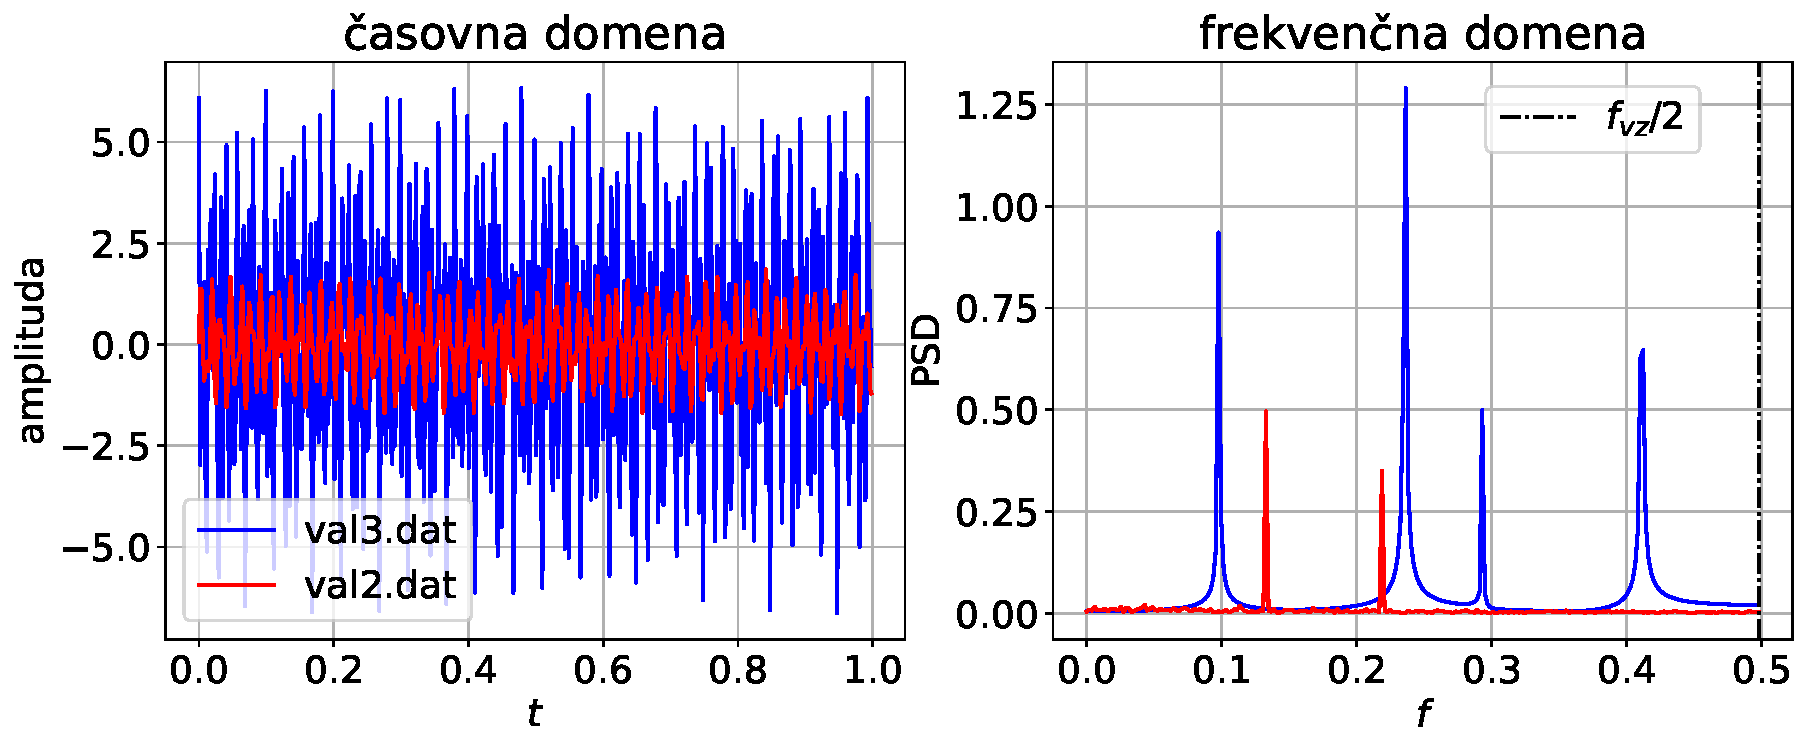
\includegraphics[width=0.7\textwidth]{10.nal_slike/surova_signala.pdf}
    \caption[short]{Surova signala}   
\end{figure}

Poskusimo uporabiti oknenske funcije za zmanjšanje puščanja. Zaradi večje nazornosti puščanja, je frekvenčni prostor prikazan v log skali. Ponovno vidimo, da puščanja na signalu 2 sploh ni. Z njim tudi hitro obupam, saj z različnimi okni signalu ne pridem do živega (se ne izboljša), dočim pri signalu 3 prihaja do očitnih sprememb. Vrh je postal mnogo ožji.

\begin{figure}[ht]
    \centering
    \begin{subfigure}{\linewidth}
        \centering
        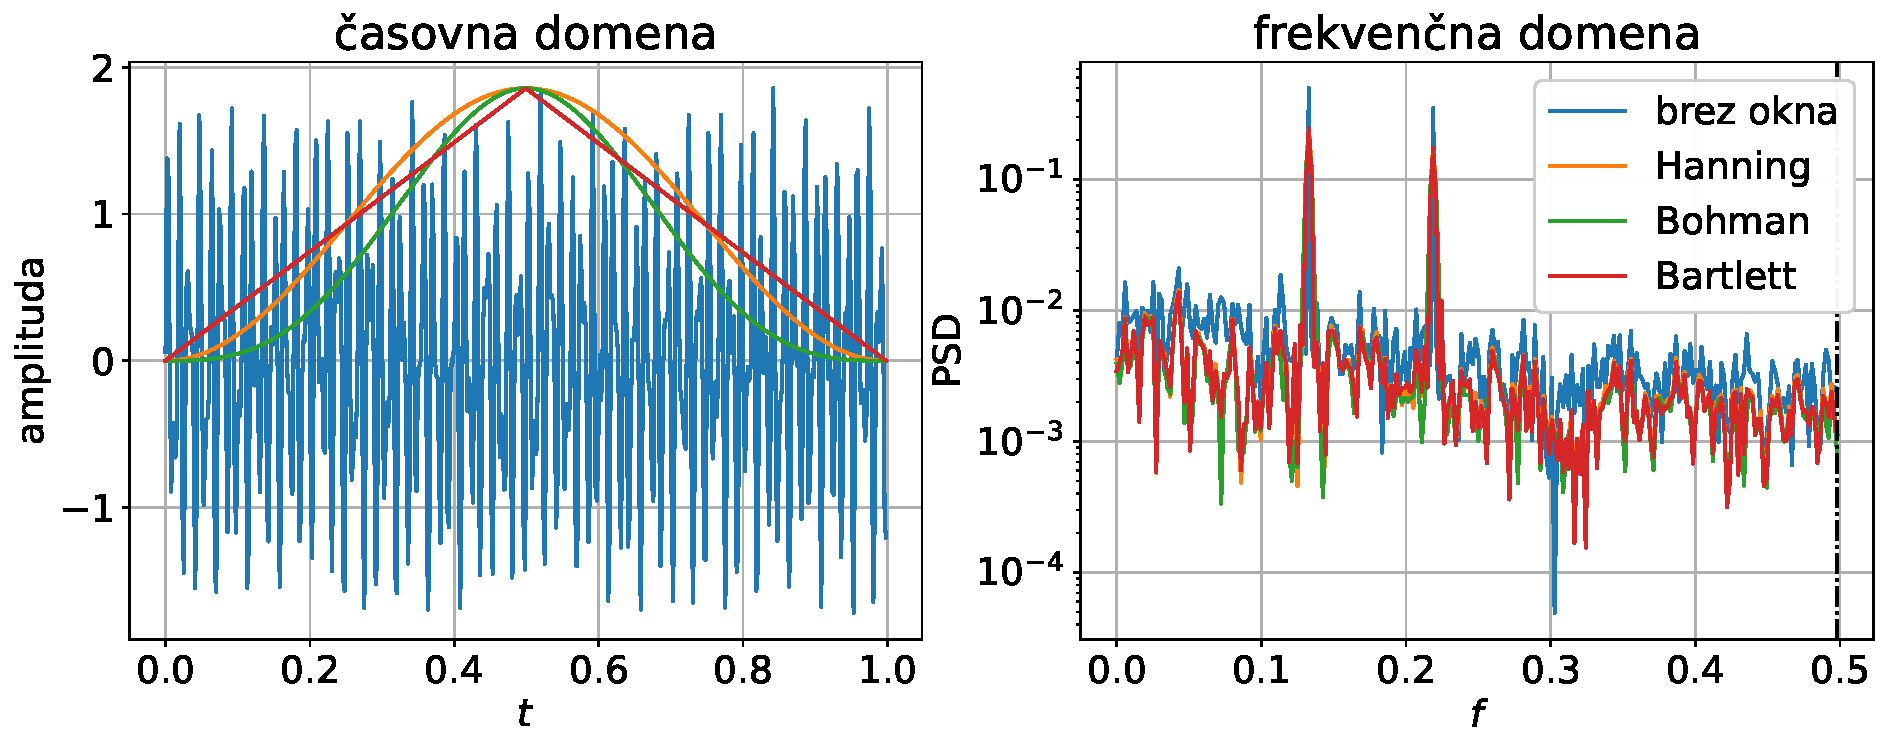
\includegraphics[width=0.6\textwidth]{10.nal_slike/okna_sig2_.pdf}
        \caption[short]{val2.dat}   
    \end{subfigure}
    \begin{subfigure}{\linewidth}
        \centering
        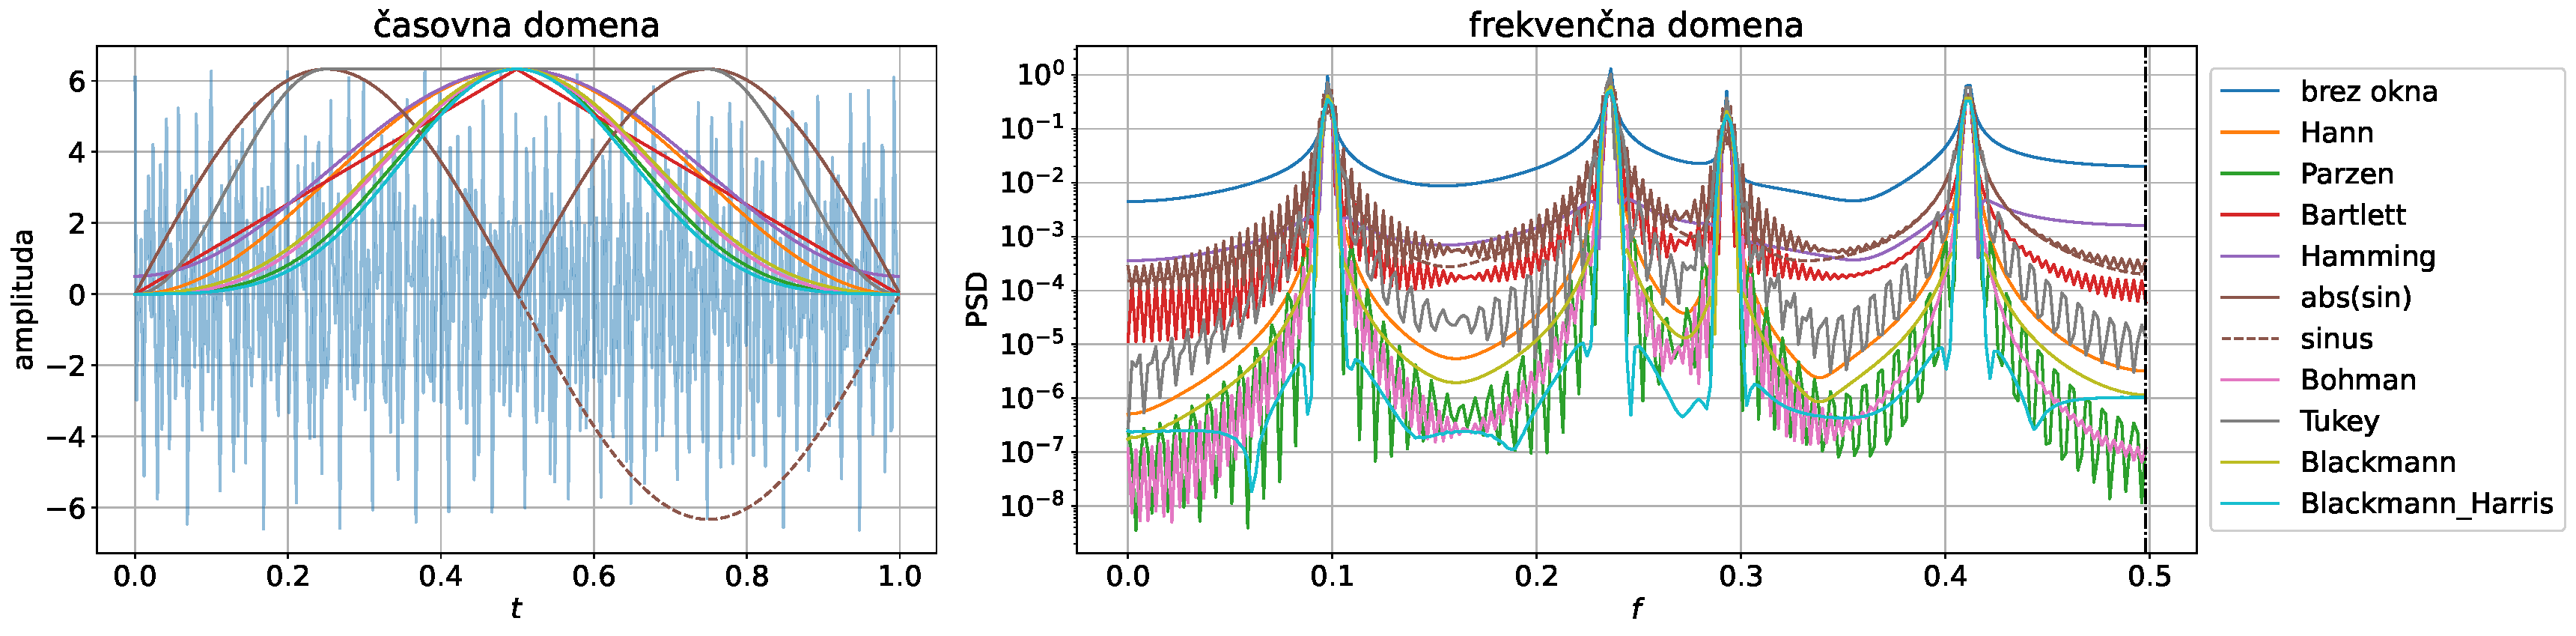
\includegraphics[width=\textwidth]{10.nal_slike/okna_sig3_.pdf}
        \caption[short]{val3.dat}
    \end{subfigure}
    \caption[short]{Analiza signalov z okenskimi funkcijami}   
\end{figure}

Opazim, da nekatera okna povzročajo oscilacije, taka v tem primeru niso uporabna. Najbolj izraziti vrhovi so pri oknu \textit{Blackmann-Harris}, vendar je pri njem prisotnih nekaj oscilacij. Gladke prehode omogočajo tudi okna \textit{Blackmann}, \textit{Hann}, \textit{sinus} in \textit{Hamming}. Zanimivo je, da moje izmišljeno okno \textit{sinus} omogoča gladke prehode vendar zajema tudi negativne vrednosti, dočim je izmišljeno okno \textit{abs(sin)} vedno pozitivno vendar vsebuje oscilacije. Domnevam, da je vir oscilacij nezvezen prehod na sredini. Vendar velja poudariti, da sta bili ti dve izmišljeni okni uspešnejši od nekaterih uveljavljenih (ki jih nisem prikazoval na grafu). \\Opomba: Še najbolje se je obnesla vizualna ocena frekvenčne domene. Apliciranje metod, ki temeljijo na razliki vrh-dolina je pri oscilirajočih primerih lahko težavno. Okarakterizacija puščnja je v splošnem težka in specifična za vsak signal.

Poizkusil sem tudi s krajšanjem signala, tako na koncu, kot tudi periodično. Opazimo, da krajšanje signala na koncu predvsem veča puščanje na signalu 3 (nisem uporabljal okenskih funkcij, vendar z njimi pričakujem podoben rezultat). Pri dovolj kratkem signalu 2 je prišlo tudi do popačenja, očitno sem zgrešil periodo signala. Če pa periodično izpuščamo podatke z izbranim korakom (tako torej višamo frekvenco vzorčenja), že zelo hitro pride do potujitve in PSD postane neuporaben.

\begin{figure}[H]
    \centering
    \begin{subfigure}{\linewidth}
        \centering
        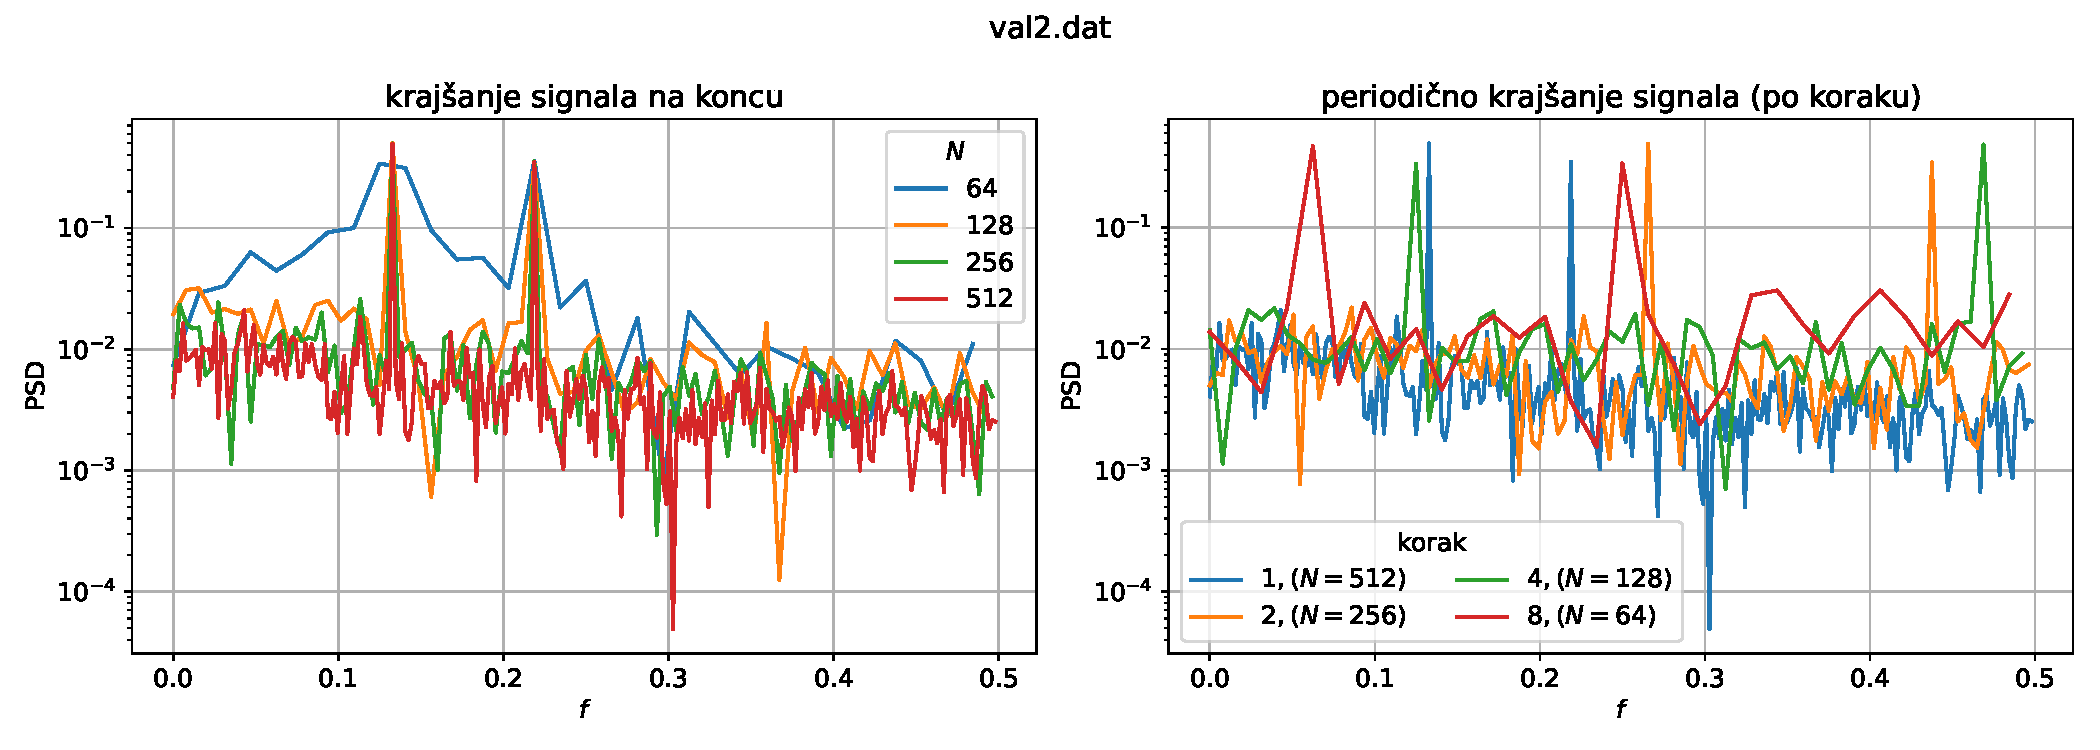
\includegraphics[width=\textwidth]{10.nal_slike/izpust_sig2.pdf}
    \end{subfigure}
    \begin{subfigure}{\linewidth}
        \centering
        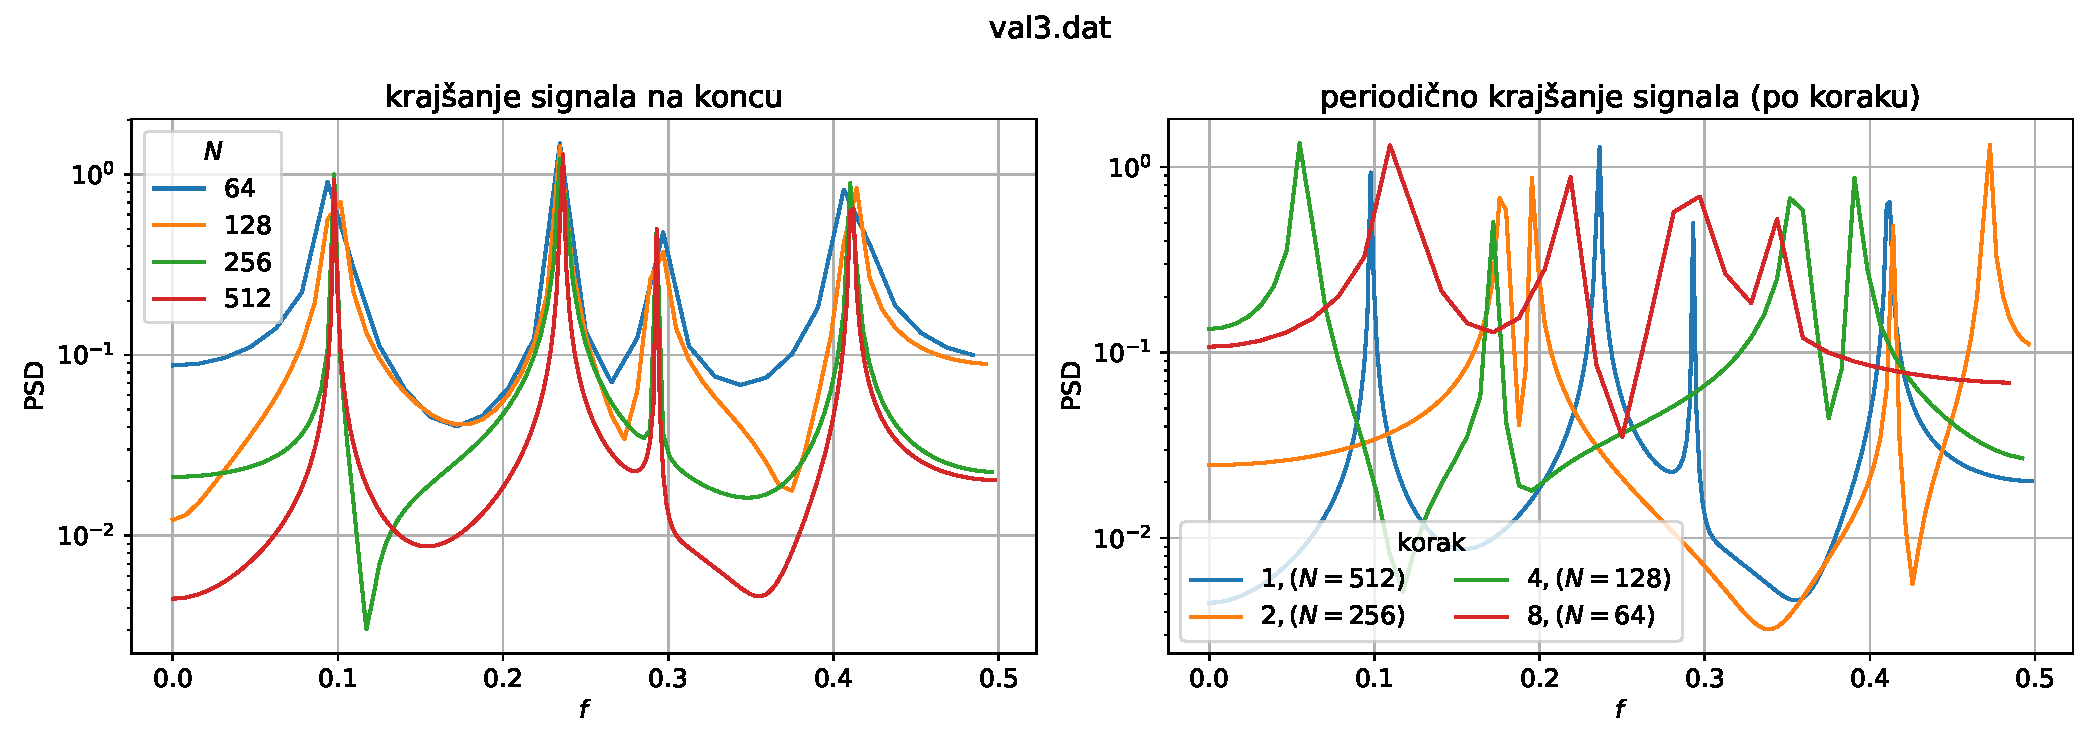
\includegraphics[width=\textwidth]{10.nal_slike/izpust_sig3.pdf}
    \end{subfigure}
    \caption[short]{Izpuščanje podatkov brez okna}   
\end{figure}

\newpage
\section{Dekonvolucija signalov z Wienerjevim filtrom}

Dekonvolucija signala $u(t)$ se lahko izvede spektralno s Fourierovo transformacijo (diskretno $\mathcal{F}_N$), če je izmerjen konvoluiran signal $c(t)$ s prenosno funkcijo $r(t)$ podan kot $ c(t) = (u*r)(t)$:
\begin{equation}
    u(t) = \mathcal{F}_N^{-1} \left[\frac{\mathcal{F}_N(c)}{\mathcal{F}_N(r)}\right] \text{.}
\end{equation}
%kjer je $u(t)$ iskani signal pred konvolucijo. 

Ker je dekonvolucija zelo občutlova na šum, uporabimo filtriranje. Tukaj se osredotočam na Wienerjev filter, ki predpostavlja, da izmerjen konvoluiran signal lahko razstavimo na dve komponenti
\begin{equation}
    c(t)  = s(t) + n(t)\text{,} \quad s(t) = (u*r)(t) \text{,}
\end{equation}
kjer je $n(t)$ šum in $s(t)$ signal brez šuma, ki ga želimo izluščiti.

Tako je Wienerjev filter
\begin{equation}
    \Phi(f) = \frac{|S(f)|^2}{|S(f)|^2+|N(f)|^2} = \frac{|C(f)|^2-|N(f)|^2}{|C(f)|^2}
\end{equation}
s katerim pomnožimo zašumljen $\mathcal{F}_N$ izmerka pred dekonvolucijo
\begin{equation}
    \tilde{u}(t) = \mathcal{F}_N^{-1} \left[\Phi(f) \, \frac{C(f)}{R(f)}\right] \text{,}
\end{equation}
pri tem so $S$, $N$, $C$ in $R$ Fourierove transformiranke $s$, $n$, $c$. in $r$ ter $\tilde{u}$ aproksimacija vhodnega signala.

dani so nam signali \texttt{signal\{0,1,2,3\}.dat}, kjer je 0 brez šuma, ostali imajo vedno večjo zašumljenost. V predlogi je podana tudi prenosna funkcija
\begin{equation}
    r(t) = \frac{1}{32} \exp{\left( -\frac{|t|}{16} \right)}
\end{equation}

Wienerjev filter je potrebno določiti ročno. V tej nalogi sem uporabljal zelo preprosto konstrukcijo Wienerjevega filtra -- določil sem mejo med področjem, kjer prevladuje šum in kjer signal ter šum utežil z nič in signal z 1. Navdušen sem bil nad tem, da tako preprost filter rešuje problem že tako dobro, da sploh nisem razmišlja o boljšem. Iz primerjave s kolegi, ki so imeli bolj sofisticirane filtre tudi na oko ni zaznati izrazitega izboljšanja. Implementacija filtrov iz knjižnice \texttt{scipy} in \texttt{skimage} se ni izkazala za uspešno.

Ker je signal0 brez šuma, je rezultat dekonvolucije že dokaj lep in potrebe po filtru ni. Vendar tudi aplikacija filtra ne pokvari rezultata in je dekonvolucija z njim tudi zelo dobra. V sledečih primerih bom podajal rezultat dekonvolucije brez šuma kot referenco!

V signalu1 je že nekaj šuma, vendar le-ta v časovni domeni ni opazen, ampak vpliva na dekonvolucijo, ki vsebuje že toliko šuma, da je neberljiva. Z malo domišljije lahko sicer izluščimo skočne funkcije. Wienerjev filter pa to težavo odpravi in dobimo manj zašumljen signal, podoben onemu iz signala0, le malenkost več je oscilacij.

Signal2 vsebuje že opazen šum, signal3 pa očitnega. Pri obeh direktna dekonvolucija odpove, wienerjev fiter pa do neke mere rešuje zadevo, saj je v tem primeru precej (še več) oscilacij.

% \begin{figure}[ht!]
%     \centering
%     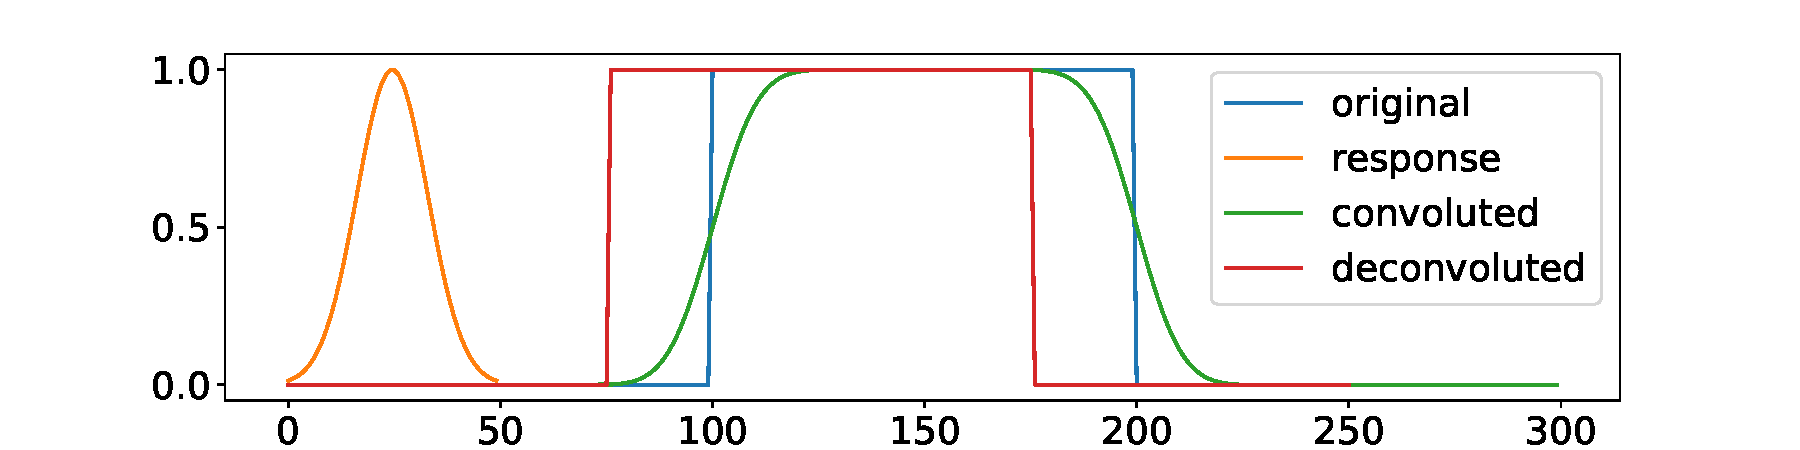
\includegraphics[width=\textwidth]{10.nal_slike/primer_dekonv.pdf}
%     \caption[short]{Primer dekonvolucije signala z vgrajenimi metodami v \texttt{scipy}}   
% \end{figure}

\newgeometry{top=1cm, bottom=2cm} %da paše slika
\begin{figure}[ht]
    \centering
    \begin{subfigure}{\linewidth}
        \centering
        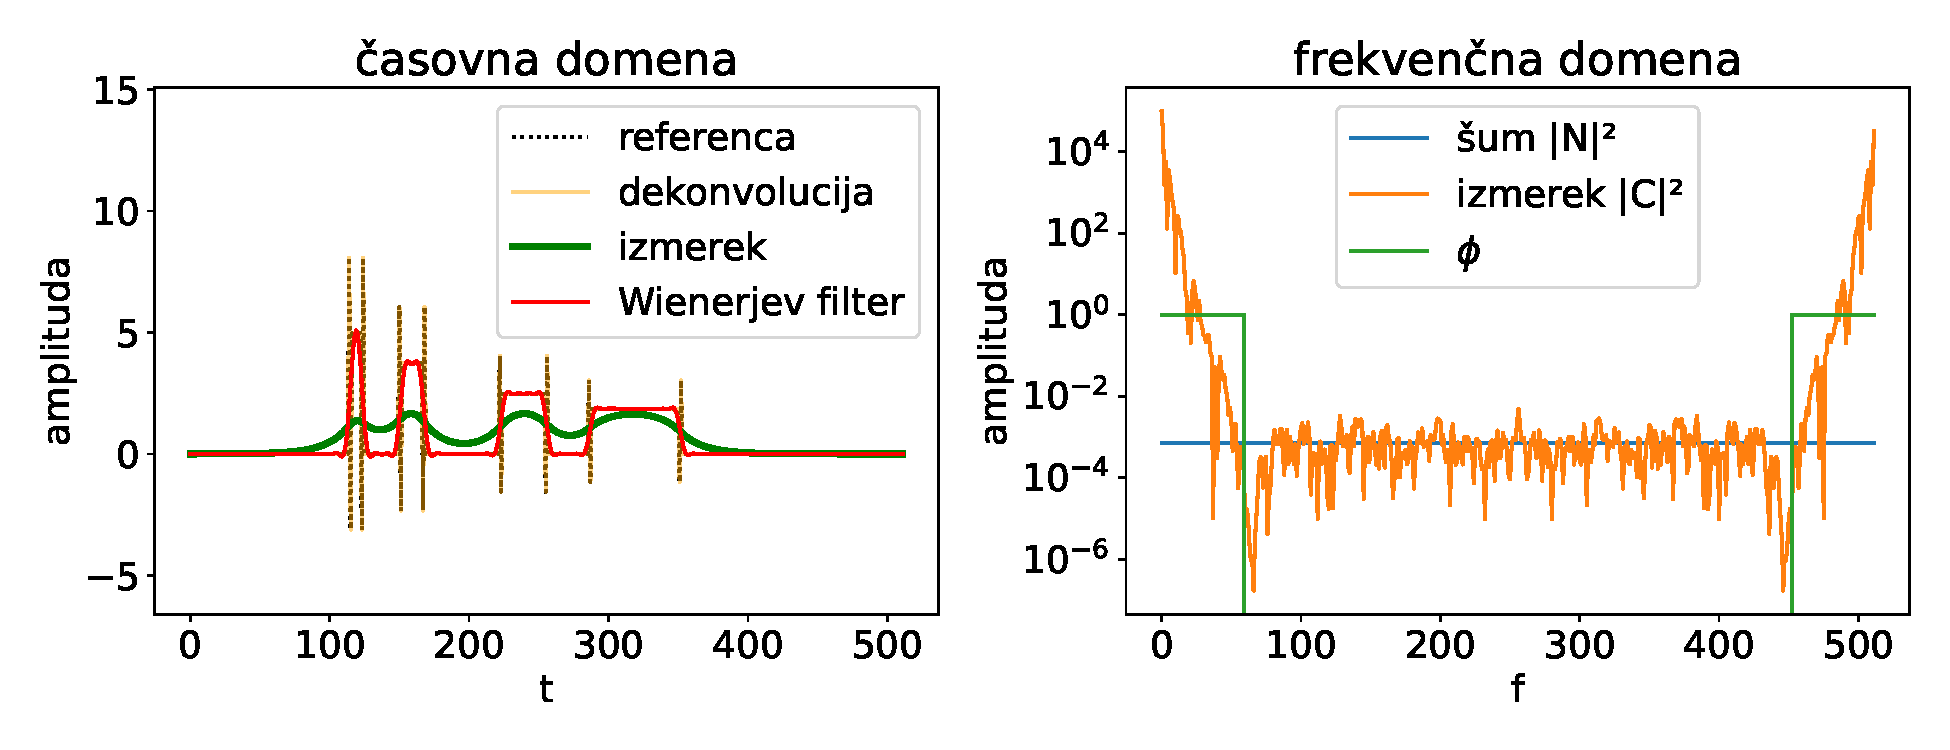
\includegraphics[width=\linewidth]{10.nal_slike/signal0.pdf}
        \caption{\texttt{signal0.dat}}
    \end{subfigure}
    \begin{subfigure}{\linewidth}
        \centering
        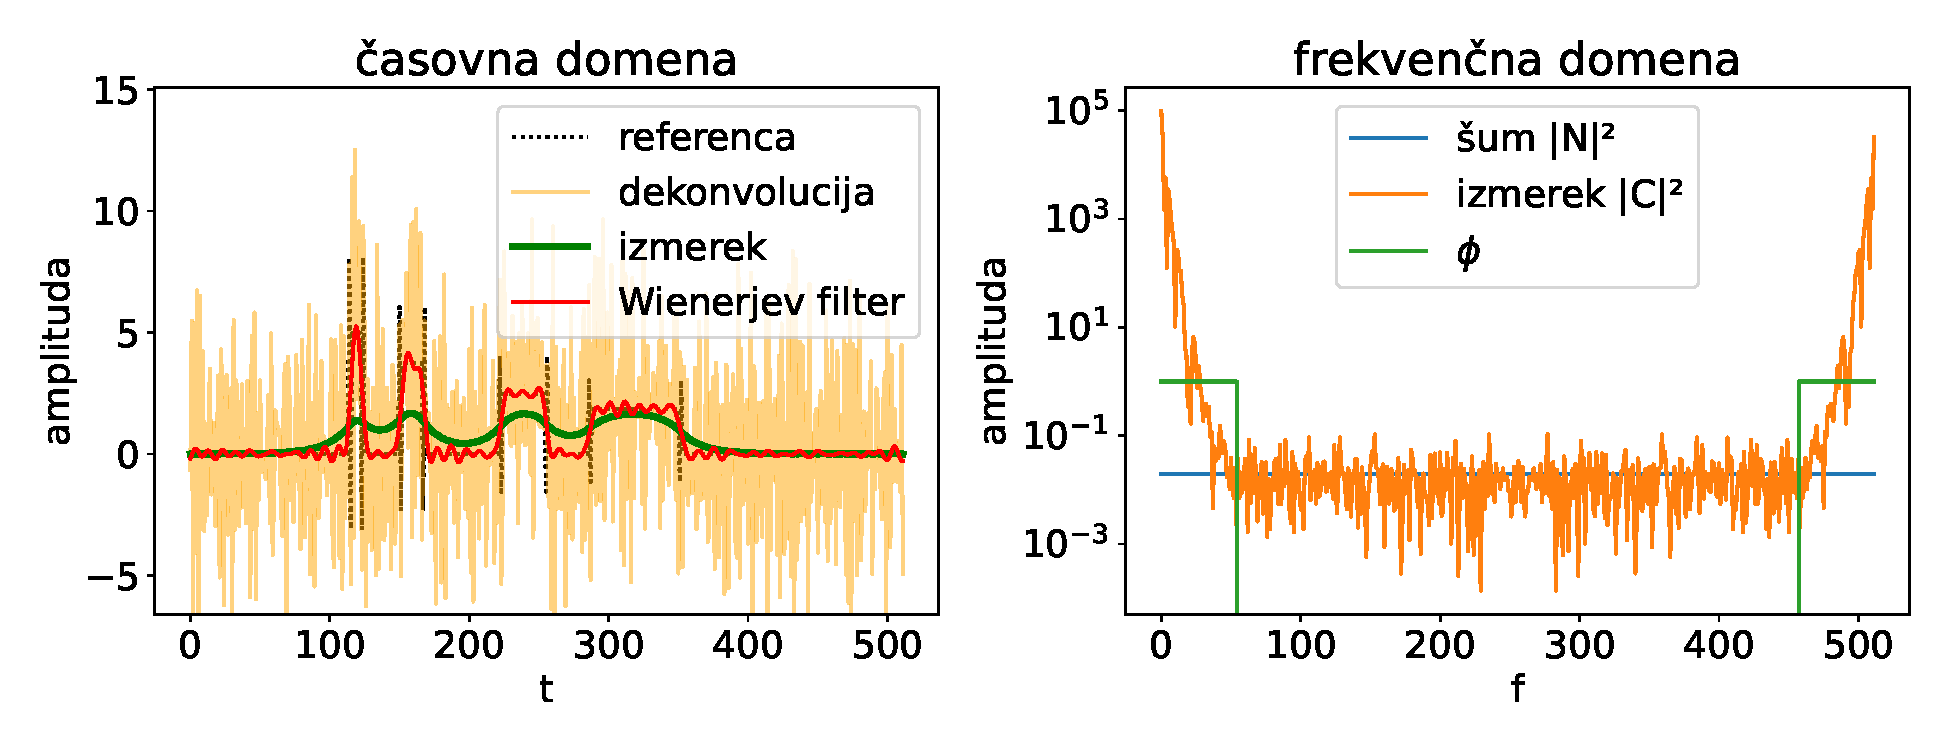
\includegraphics[width=\linewidth]{10.nal_slike/signal1.pdf}
        \caption{\texttt{signal1.dat}}
    \end{subfigure}
    \begin{subfigure}{\linewidth}
        \centering
        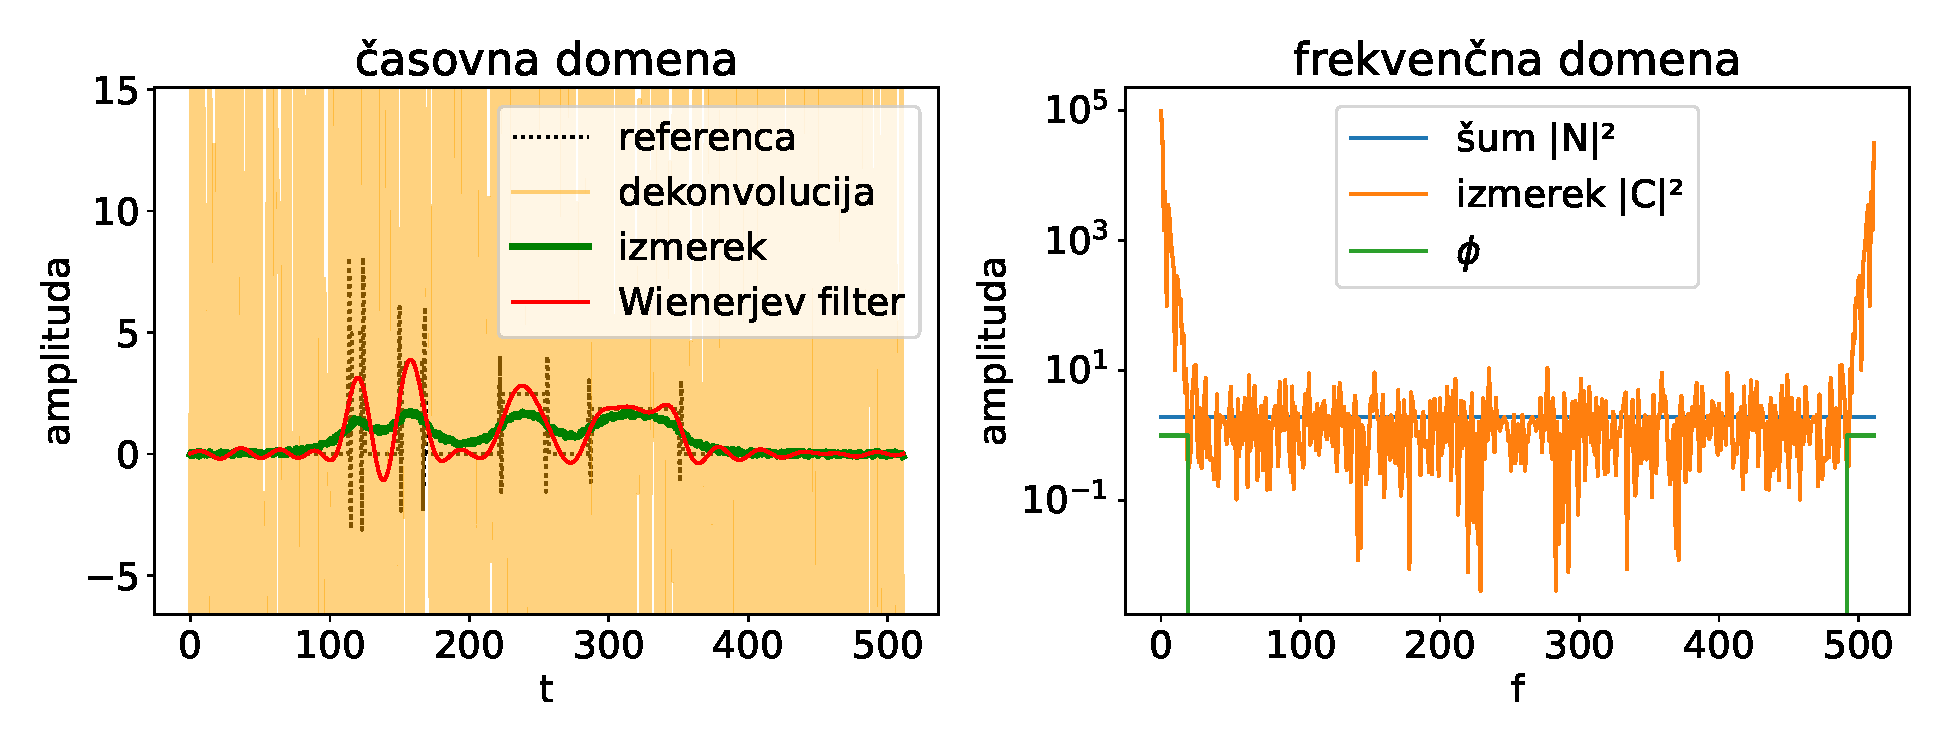
\includegraphics[width=\linewidth]{10.nal_slike/signal2.pdf}
        \caption{\texttt{signal2.dat}}
    \end{subfigure}
    \begin{subfigure}{\linewidth}
        \centering
        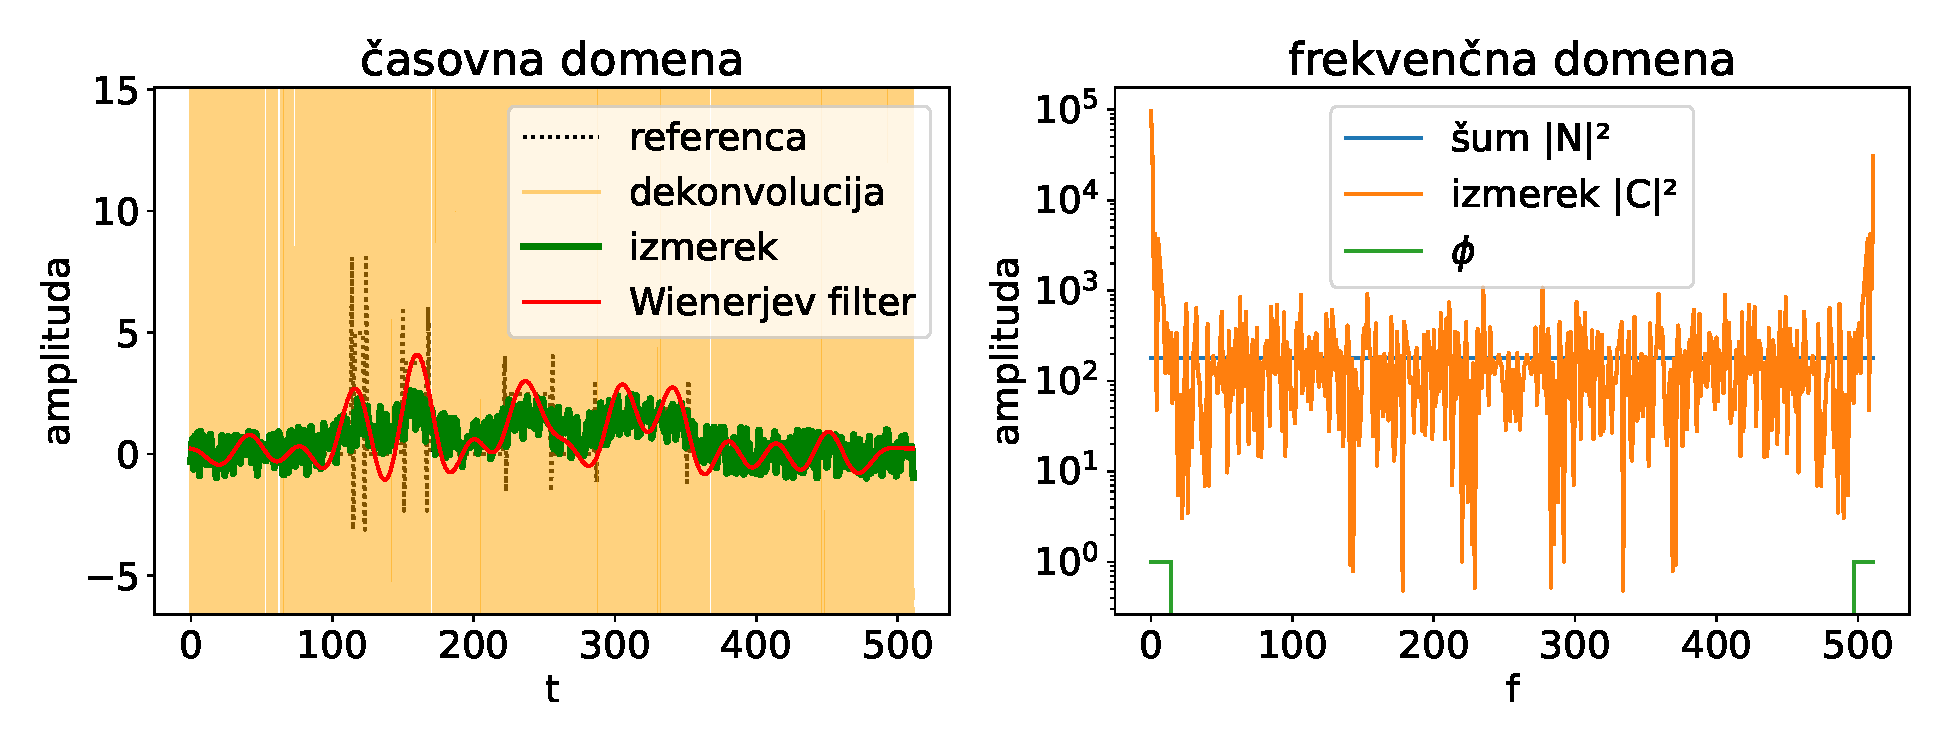
\includegraphics[width=\linewidth]{10.nal_slike/signal3.pdf}
        \caption{\texttt{signal3.dat}}
    \end{subfigure}
    \caption{Dekonvolucija signalov z Wienerjevim filtrom}
\end{figure}
\restoregeometry % Restore original margins

\section{Rekonstrukcija fotografije}

Podane so slike \href{https://en.wikipedia.org/wiki/Lenna}{Lene}, razmazane s različnimi konvolucijskimi jedri/kernel (na sliki spodaj) in različnimi količinami Gaussovskega šuma. 

\begin{figure}[ht]
    \centering
    \begin{subfigure}{0.3\linewidth}
        \centering
        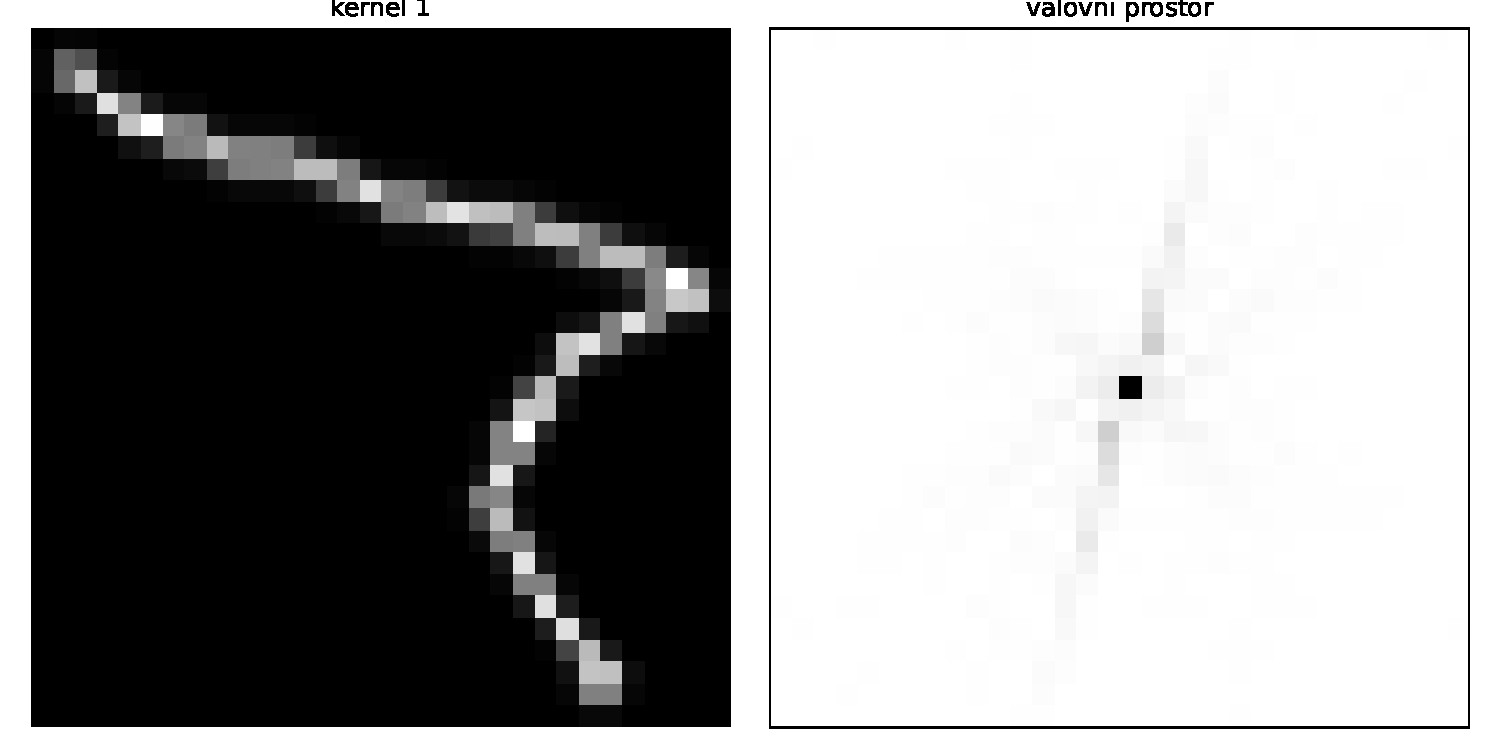
\includegraphics[width=\linewidth]{10.nal_slike/10.3/kernel1.pdf}
        \caption{Jedro 1: tresoč objektiv}
    \end{subfigure}\hfill
    \begin{subfigure}{0.3\linewidth}
        \centering
        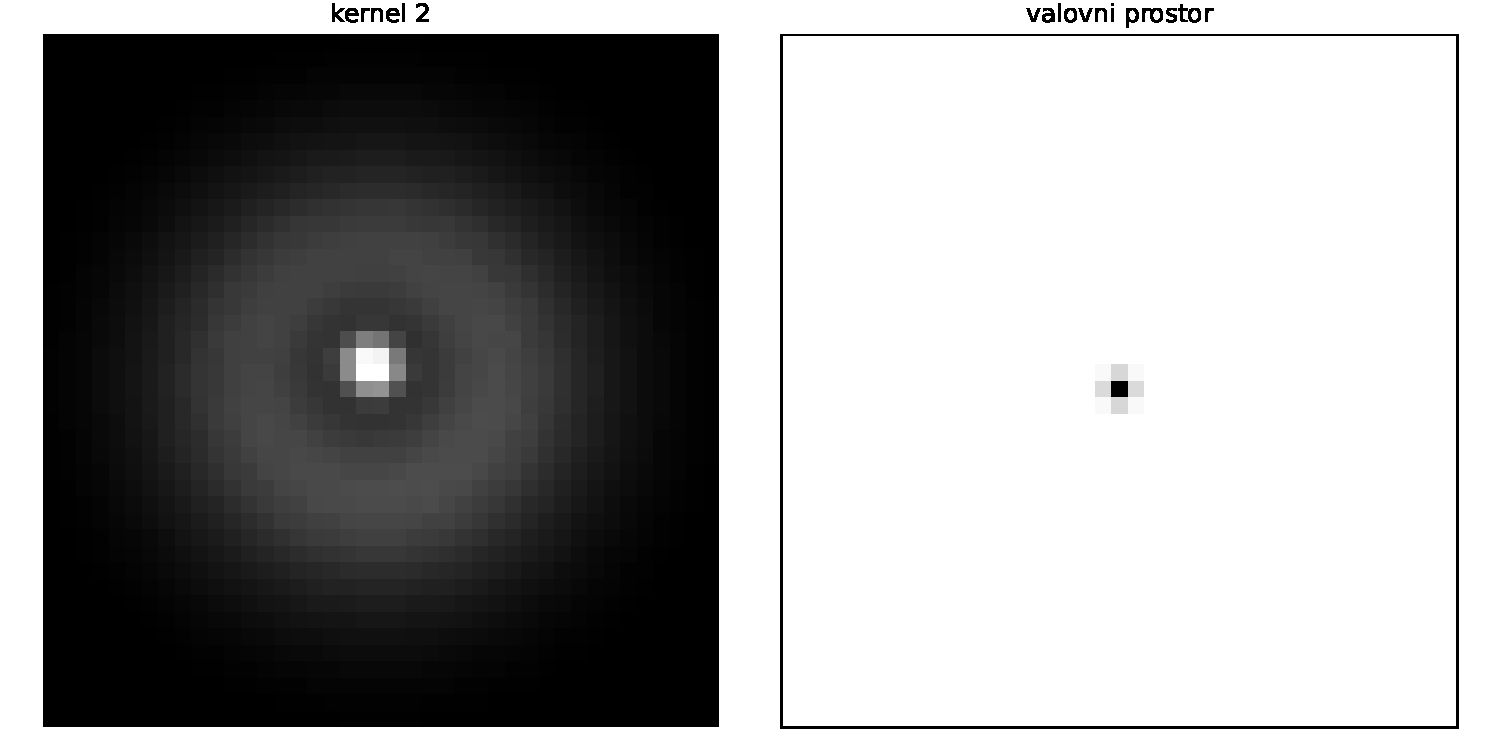
\includegraphics[width=\linewidth]{10.nal_slike/10.3/kernel2.pdf}
        \caption{Jedro 2: slab fokus}
    \end{subfigure}\hfill
    \begin{subfigure}{0.3\linewidth}
        \centering
        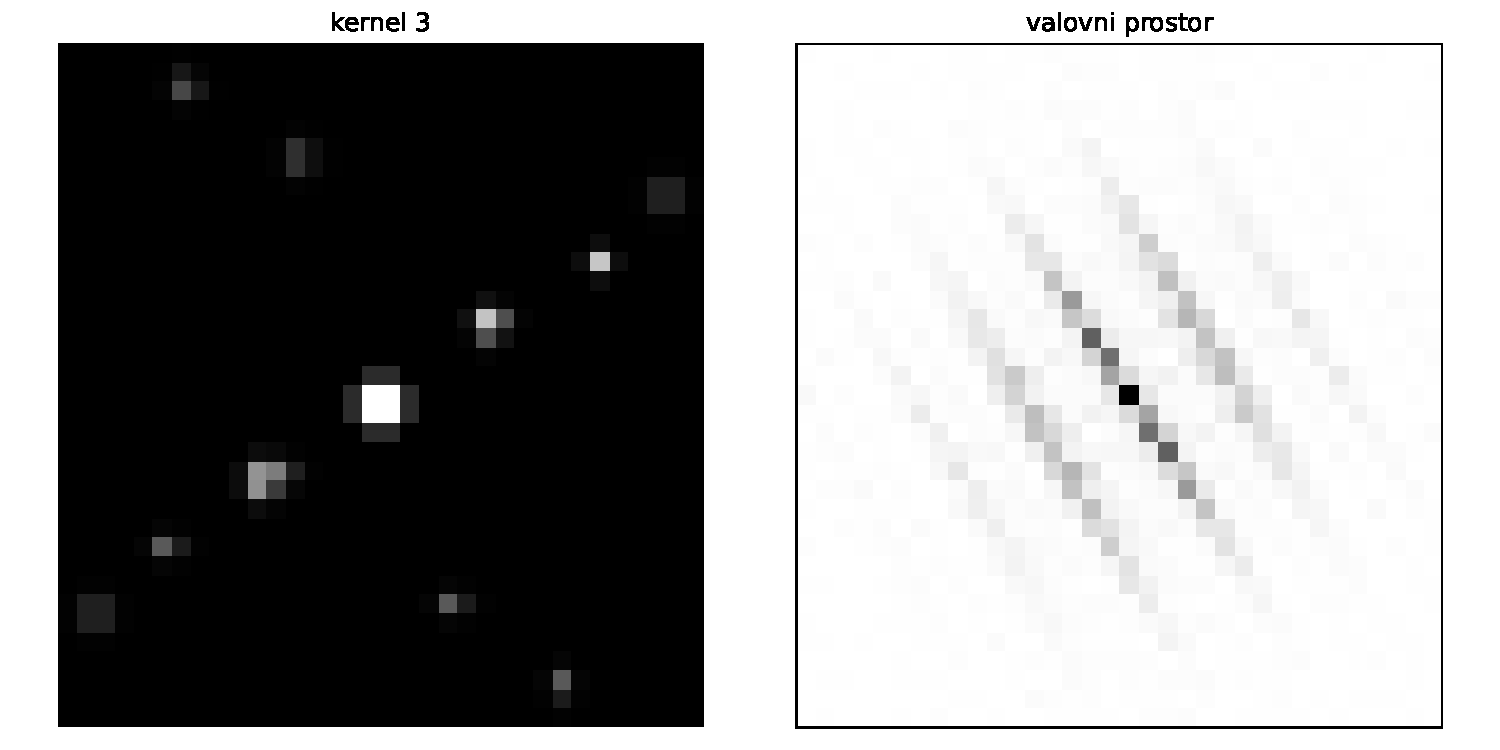
\includegraphics[width=\linewidth]{10.nal_slike/10.3/kernel3.pdf}
        \caption{Jedro 3: ukl. mrežica}
    \end{subfigure}
    \caption{Konvolucijska jedra}
\end{figure}

Problem dekonvolucije se rešuje na podoben princip kot v prejšnjem poglavju, le da tokrat uporabljamo FFT v dveh dimenzijah. Kot prvo sem poizkusil rekonstruirati kernel 1 brez šuma in kmalu ugotovil, da dekonvolucijo zmoti rob slike, zato sem uporabil različne okenske funkcije, kar pa močno zatemni sliko, čemur sem dodal različno število pikslov (px) po robu na načine, predstavljene na spodnji sliki. Opomba: dodatek px konstantne vrednosti je ekvivalenten nerazširjeni sliki; zaradi narave kode, brez dodatka ni šlo.

\begin{figure}[H]
    \centering
    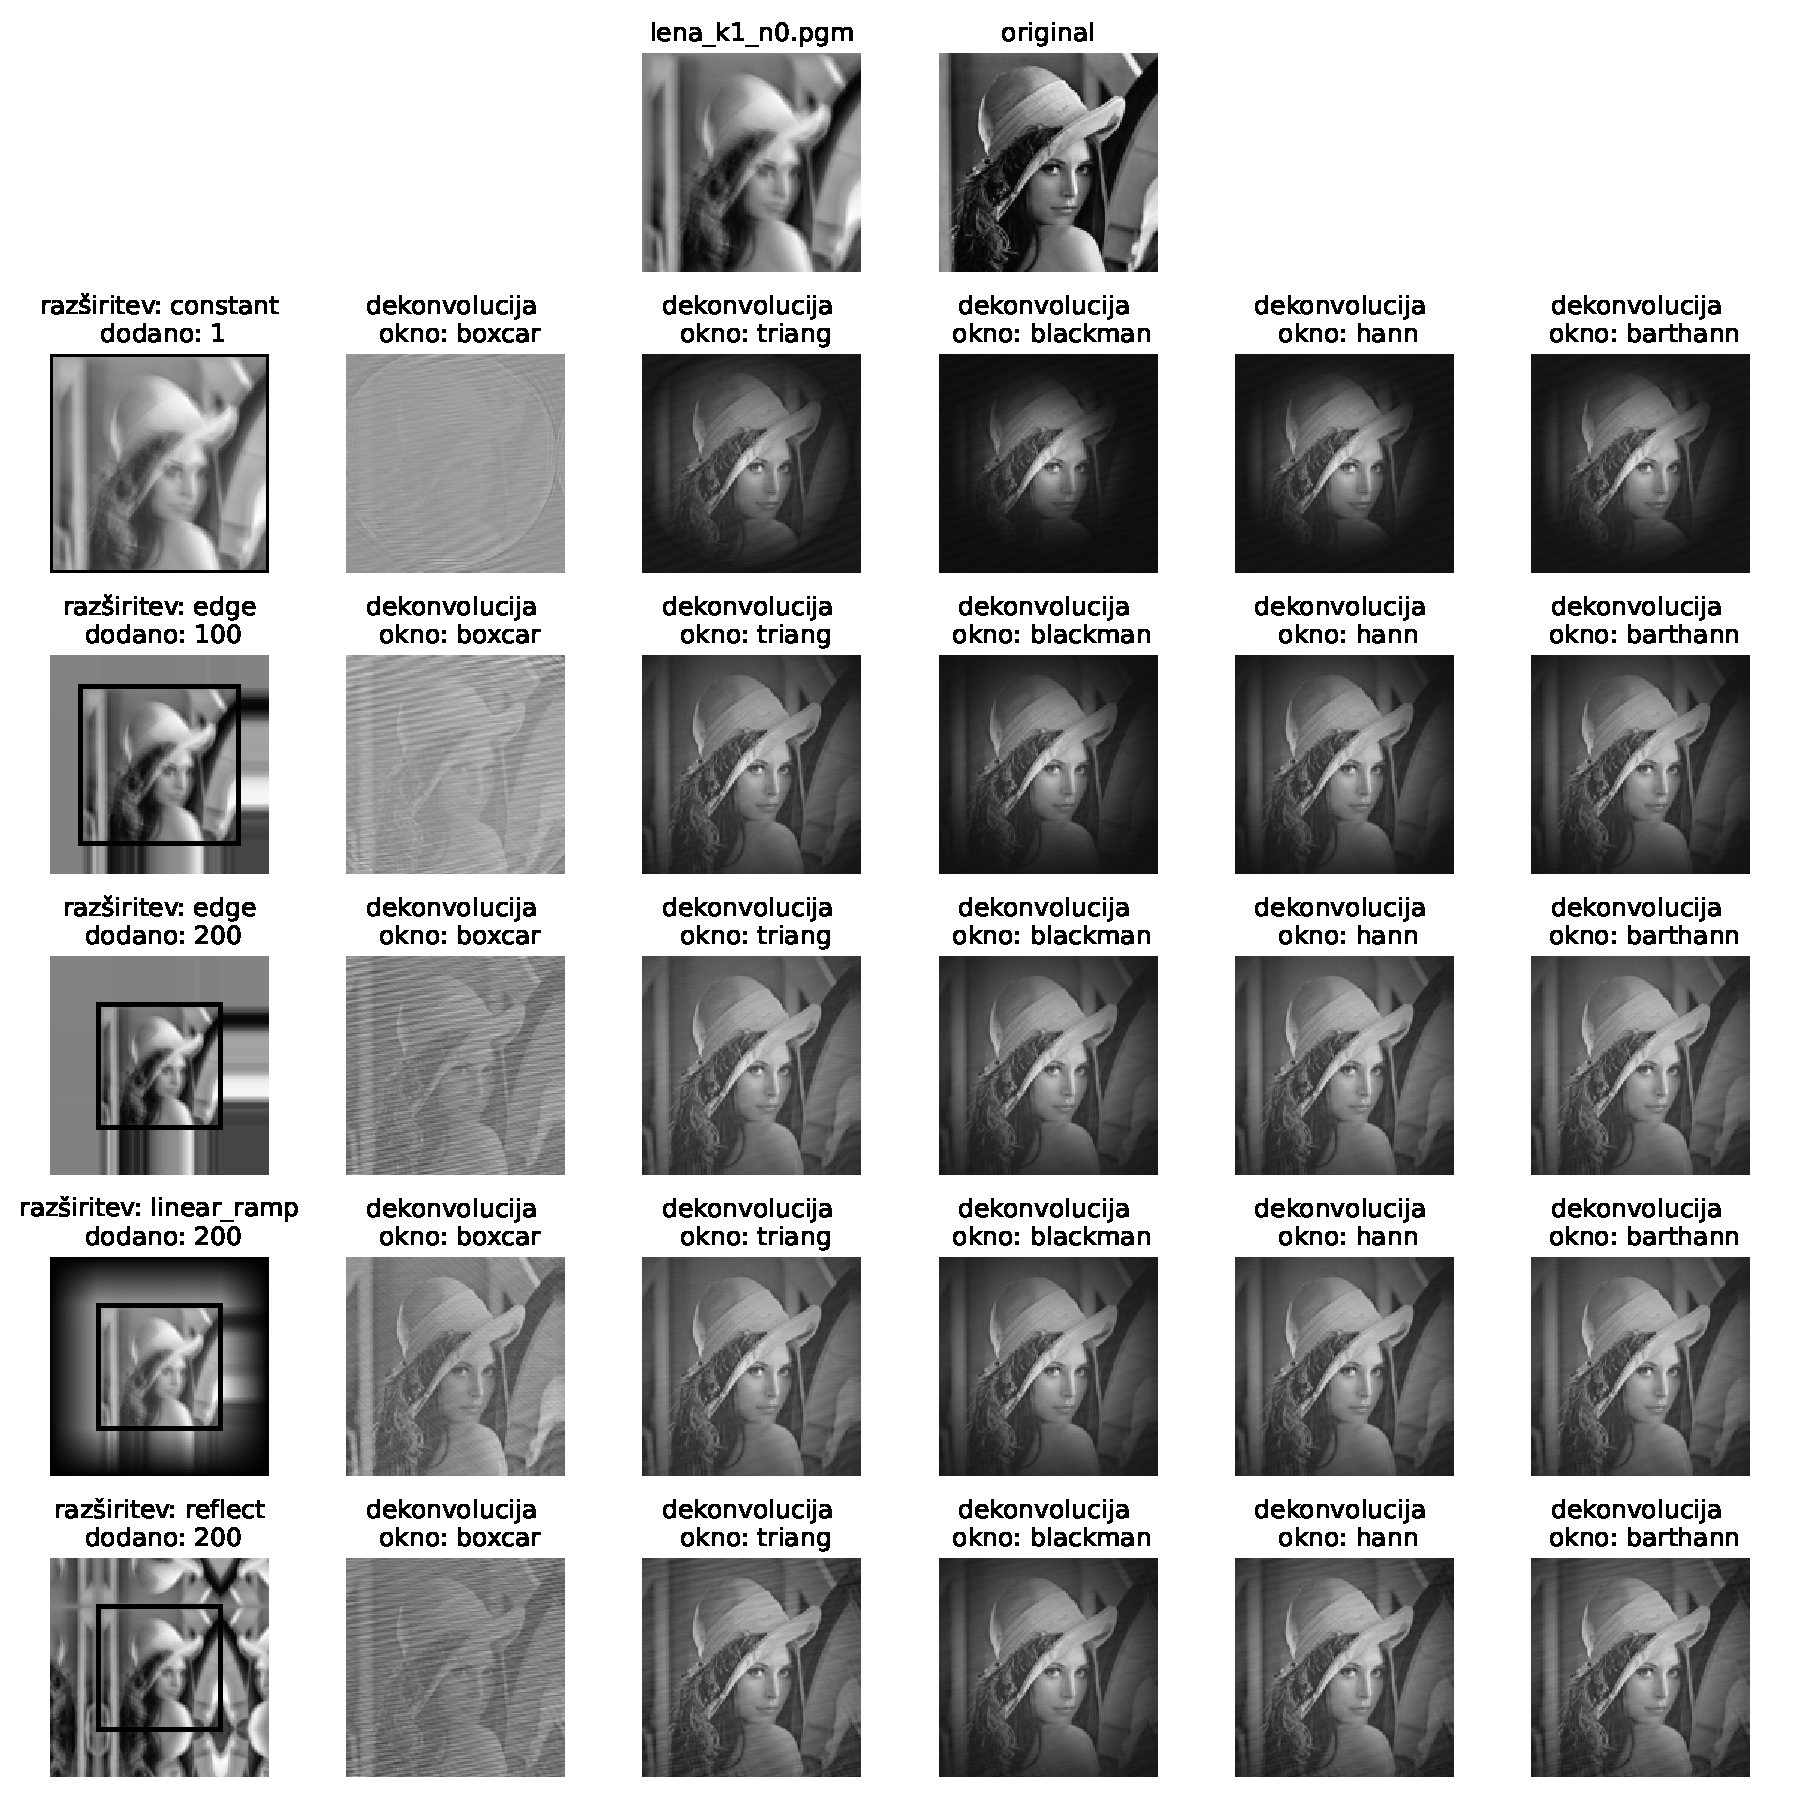
\includegraphics[width=\textwidth]{10.nal_slike/10.3/kernel1_dekonv_okna.pdf}
    \caption{Dekonvolucija slike \texttt{lena\_k1\_n0.pgm} z različnimi okni in razširitvami}   
\end{figure}

Ugotovil sem, da dodatek 200 px sliko močno izboljša, skupaj z uporabo primerne okenske funkcije (okna). Izgleda da se najbolje obnese razširitev \textit{linear ramp}, vendar razlike vizualno niso tako očitne pri uporabi okenskih funkcij (opomba: \textit{boxcar} je naziv za okno konstantne vrednosti 1, torej kot bi okenske funkcije ne bilo!). Nekatera okna zelo zatemnijo sliko, zato tu niso prikazana. Vizualno lahko sklepam, da je dodatek 200 px razširitve linear ramp in okna triang (Bartlett), Hann, Barthann najugodnejše.

V modulu \texttt{skimage.restoration} sem našel implementacijo algoritma \textit{Richardso-Lucy} (LR), ki ob znani PSI (point spread function), kar je naš kernel, poskuša iterativno povrniti (dekonvoluirati) originalno sliko. Kot je razvidno iz spodnje slike, je pri tem algoritem precej uspešen, sploh če mu pomagamo z razširitvijo slike, kot pri klasični dekonvoluciji. Pri nerazširjeni sliki so artefakti na robu lepo vidni, pri prevelikem številu iteracij pa prihaja do popačenja, ki se kot valovi širi preko celotne slike, če še dodatno večamo število iteracij. To se venomer zgodi v spodnjem levem robu in izgleda, kot da bi se algoritem ``ujel v Lenine lase''. Izkaže se, da nekako 50 iteracij vrne zadovoljiv rezultat, ki se nadaljno ne izboljšuje pretirano. Potrebno je poudariti, da je ta algoritem tudi bolj računsko zahteven od naše spektralne metode.

\begin{figure}[ht]
    \centering
    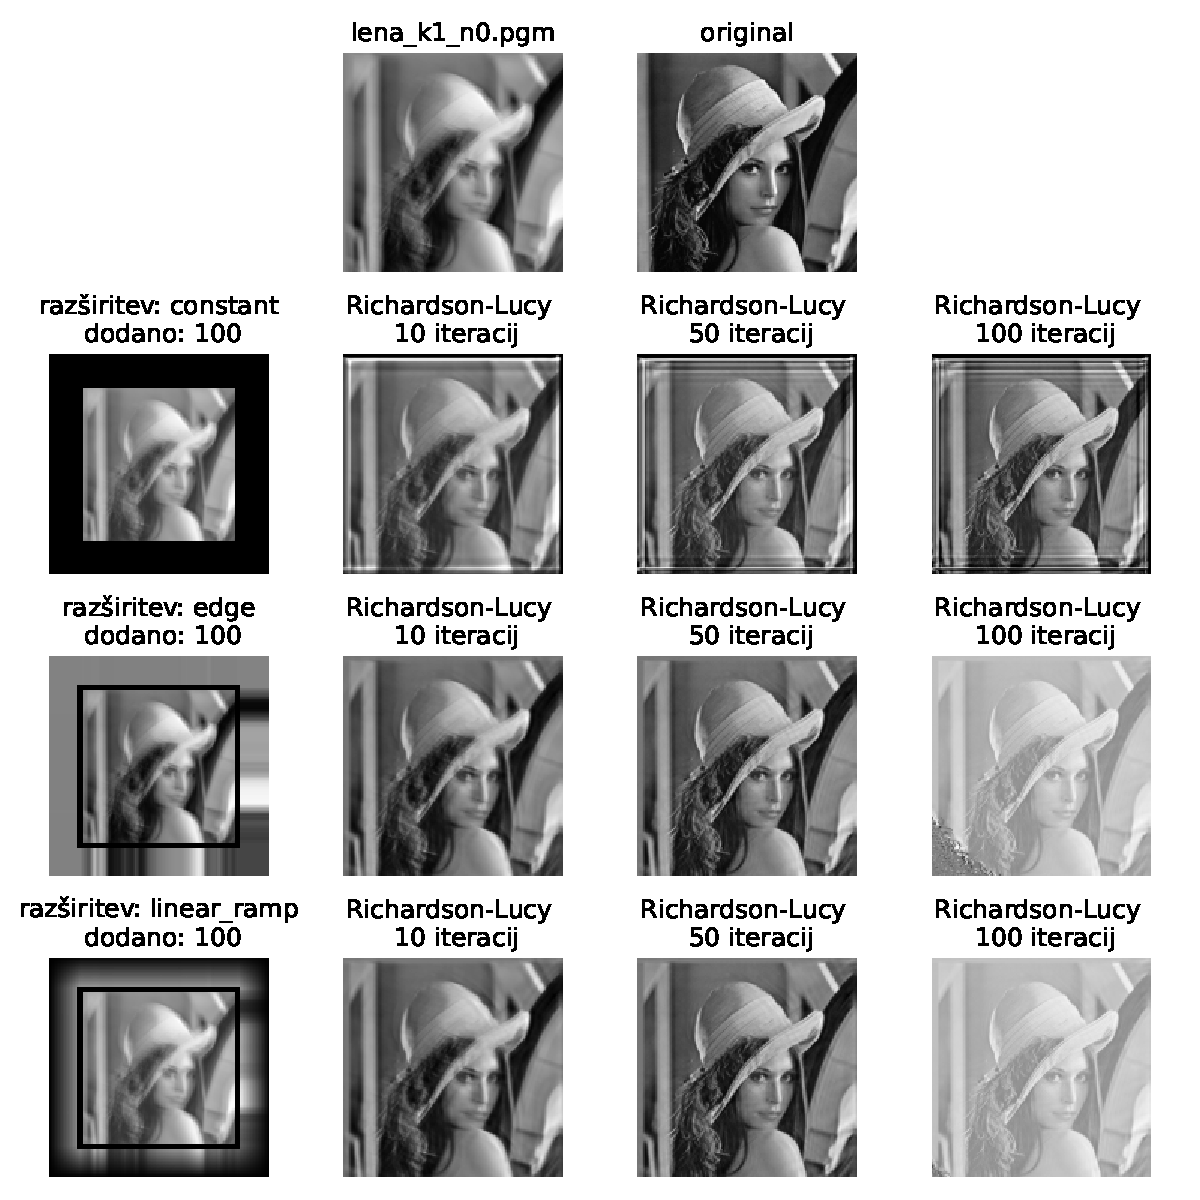
\includegraphics[width=\textwidth]{10.nal_slike/10.3/kernel1_dekonv_LR.pdf}
    \caption{Dekonvolucija slike \texttt{lena\_k1\_n0.pgm} z različnimi razširitvami in iteracijami}   
\end{figure}

\newpage
Da lahko bolje ovrednotim rezultate, sem uporabil \href{https://www.researchgate.net/figure/The-famous-Lena-image-often-used-as-an-example-in-image-processing_fig1_235673010}{originalno sliko} in jo pretvoril v grayscale zapis, s katerim sem primerjal rezultate dekonvolucije na sledeč način:
\begin{equation}\label{eqn:eta}
    \eta = \frac{|| D_{ij} - R_{ij} ||}{|| S_{ij} - R_{ij} ||},
\end{equation}
kjer so $R$, $D$ in $S$ matrike referenčne(originalne), dekonvoluirane in signalne(podane) slike. Torej, če z dekonvolucijo slike nismo čisto nič izboljšali, je vrednost relativne napake $\eta$ obdelane slike 100\%, če smo pa uspeli popolnoma rekonstruirati original, pa ima $\eta$ vrednost nič.

Za primere, prikazane v zgornjih dveh slikah lahko  izračunamo vrednosti relativnega odstopanje od originala v odvisnosti od števila dodanih px ($N_{add}$). Ugotovim podobno, kot sem sklepal vizulano; najhitreje pade napaka pri oknu triang, vendar se kasneje razlike med okni zmanjšajo. Edino brez okna (boxcar) se obnaša nepredvidljivo, a ne da uporabnih rezultatov. Razlike med tipi razširitev niso tako velike pri manjših razširitvah, linear-ramp in endge sta celo identični (velja le za okno triang!), dočim je rezultat za algoritem LR presenetljiv. Tega v tem trenutku ne znam pojasniti. Prav tako sem pričakoval, da bo pri iteracijah nad 100 prišlo do poslabšanja, vendar je začuda
temu ravno obratno. Algoritem LR sicer vrne malenkost manj ostro sliko, vendar bolj kontrastno od dekonvolucije.
\\ Opombi: Število iteracij pri LR se na grafu prične z 1 zaradi tehničnih razlogov. Pri opazovanju napak datotek \texttt{lena\_k2\_n0.pgm} in \texttt{lena\_k3\_n0.pgm} je potek drugačen (predvsem za algoritem LR)!

\begin{figure}[ht]
    \centering
    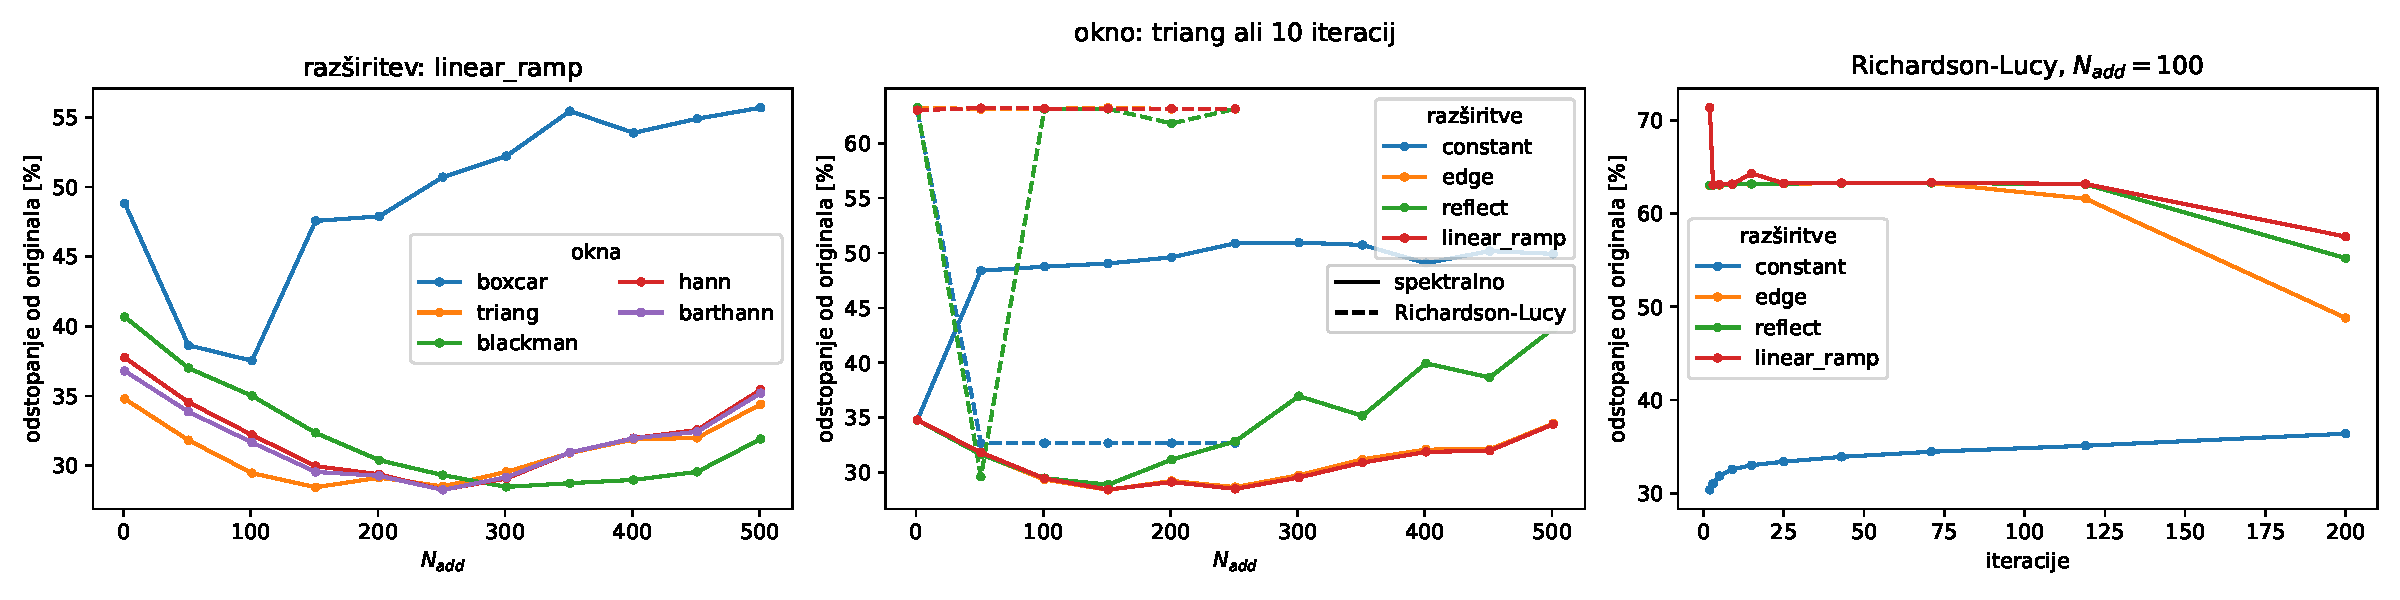
\includegraphics[width=\textwidth]{10.nal_slike/10.3/napaka_kernel1.pdf}
    \caption{Napaka dobljene slike glede na pravo Leno za datoteko \texttt{lena\_k1\_n0.pgm}}
    \label{fig:napaka}
\end{figure}

Najbolj perspektivno za obravnavo se izkaže okno triang in razširitev linear-ramp med 150 in 250 px. Omeniti velja, da manjša razširitev pohitri izračun, prav tako pa je potrebnih manj iteracij LR. Do sedaj sem obravnaval le datoteko \texttt{lena\_k1\_n0.pgm} in ugotovil, kaj se dobro obnese, sedaj po bom te metode poskušal aplicirati tudi na preostalih dveh slikah brez šuma.

Za lažjo nadaljno obravnavo lahko določimo nov parameter ujemanja rekonstruirane slike z originalom
\begin{equation}
    1-\eta.
\end{equation}
Tukaj $\eta$ izračunamo po enačbi \ref{eqn:eta}. Vrednost 1 pomeni popolno ujemanje z originalom, 1 pa brez izboljšave. 

Sedaj lahko napademo še preostali dve sliki brez šuma, kjer uporabimo okno triang, razširitev linear-ramp z 200 px in 50 iteracij. Domnevam, da je zaradi narave jedra 2 (tresoč objektiv), ki spominja na Gaussovski šum, direktna dekonvolucija neuspešna, na jedru 3 pa deluje uspešno. Algoritem LR daje primerljive rezultate na jedru 1, navkljub (ponovno čudno) nizkim izračunom ujemanja. Na jedru 2 se obnese odlično v primerjavi z dekonvolucijo. Potrebno je opomniti, da vrne algoritem LR na jedru 3 boljše rezultate pri manj iteracijah, nekako med 10 in 20, kar je uporabljeno v prilogi, vendar rezultati LR vseeno niso primerljivi z dekonvolucijo.

\begin{figure}[H]
    \centering
    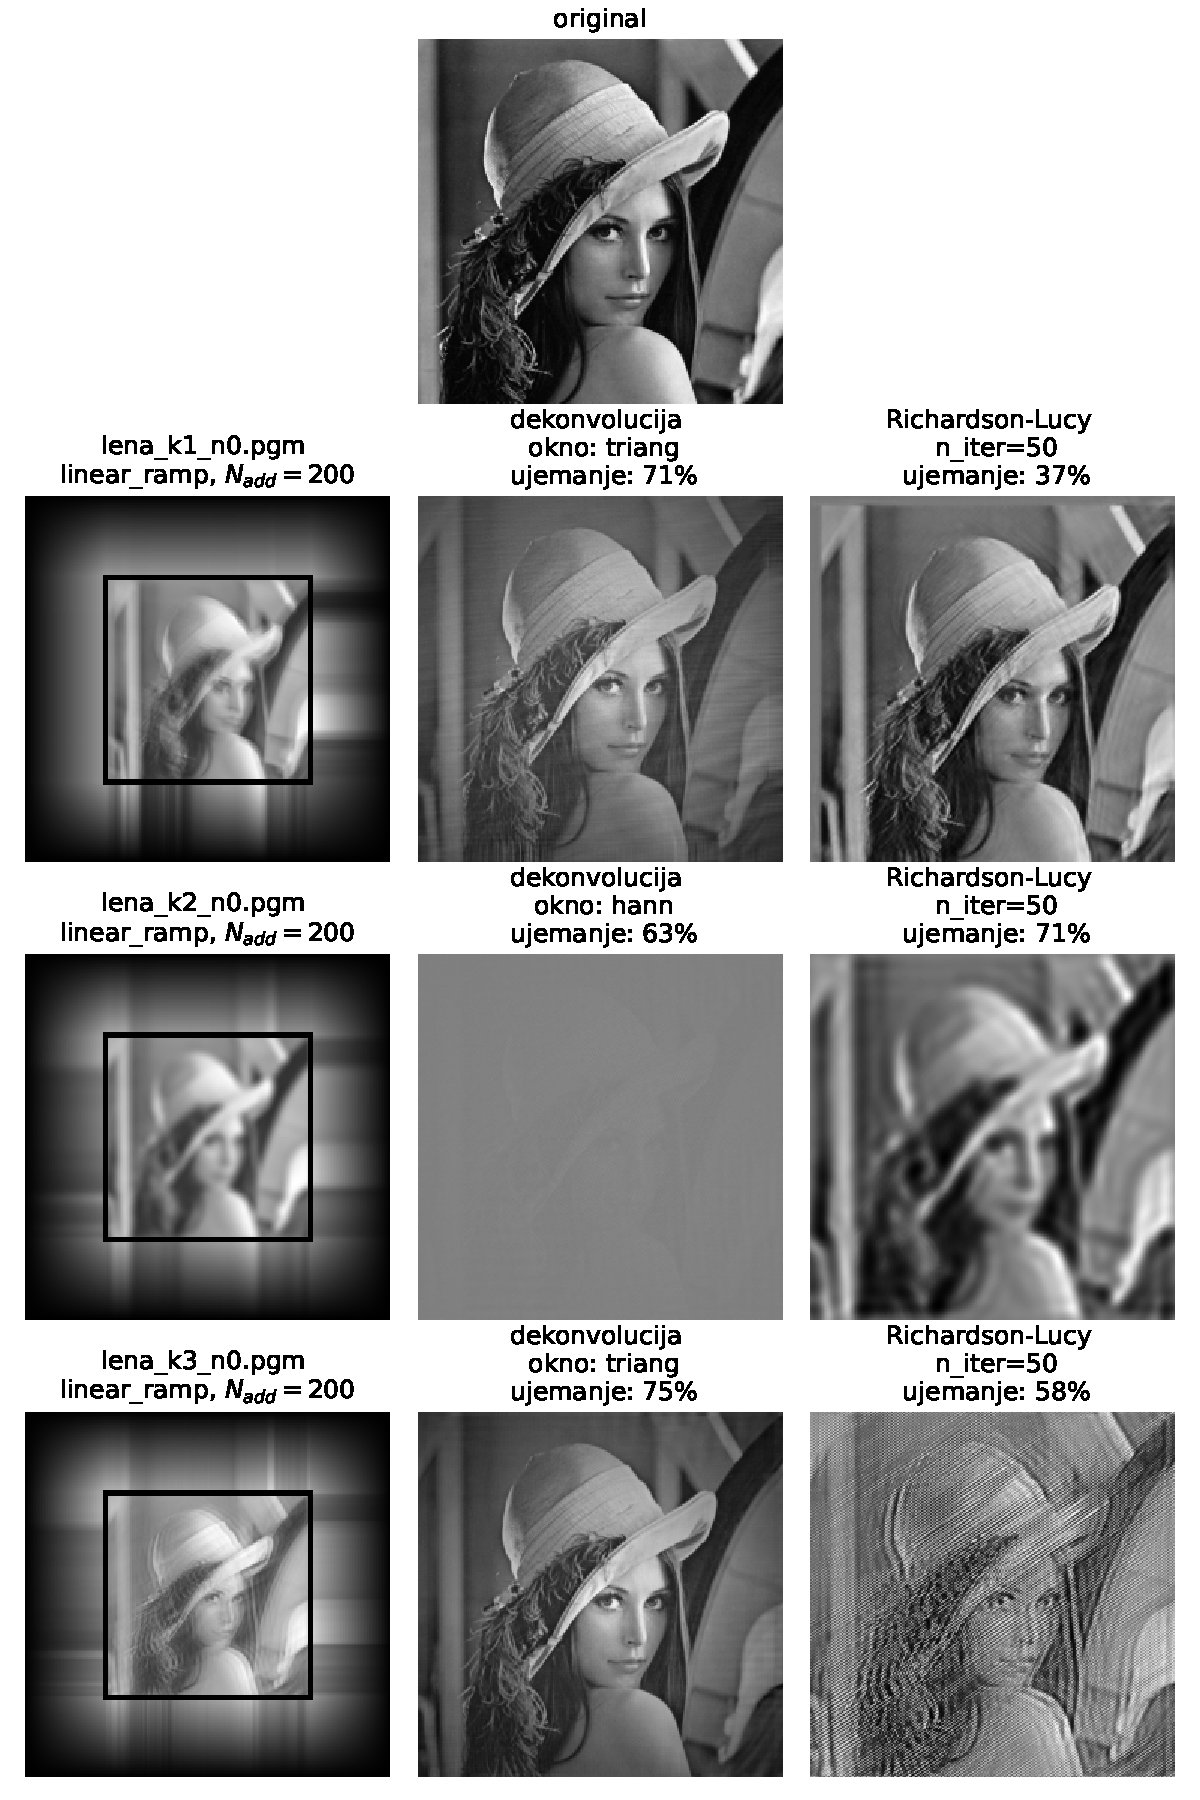
\includegraphics[width=0.6\textwidth]{10.nal_slike/10.3/dekonv_vsa_jedra.pdf}
    \caption{Dekonvolucija preostalih slik brez šuma z najboljšimi okni in razširitvami}   %kernel3 algoritem LR se bolje obnese z manj iteracijami (10-20)
    \label{fig:vse_brez_sum}
\end{figure}

Za analizo slik z dodanim Gaussovskim šumom moramo ponovno uporabiti filter. Naš delovni konj je v tem primeru Wienerjev filter. Uporabljam filter z Wiener-Hunt-ovim pristopom iz knjižnice \texttt{skimage.restoration}, ki je spisan za n-dimenzij. S parametrom \textit{balance} omogoča, da krmilimo med obnovitvijo podatkov in artefaktom zaradi šuma. Na primeru jedra 1 in RMS šuma 4 je to prikazano na spodnji sliki. Opazimo, da se slika vidno izboljšuje do nekje $10^6-10^7$, dalje se sicer ujemanje veča, vendar slike opazno izgublja ostrino, zato na tem mestu lahko dvomim o ustreznosti parametra ujemanja!

\begin{figure}[ht]
    \centering
    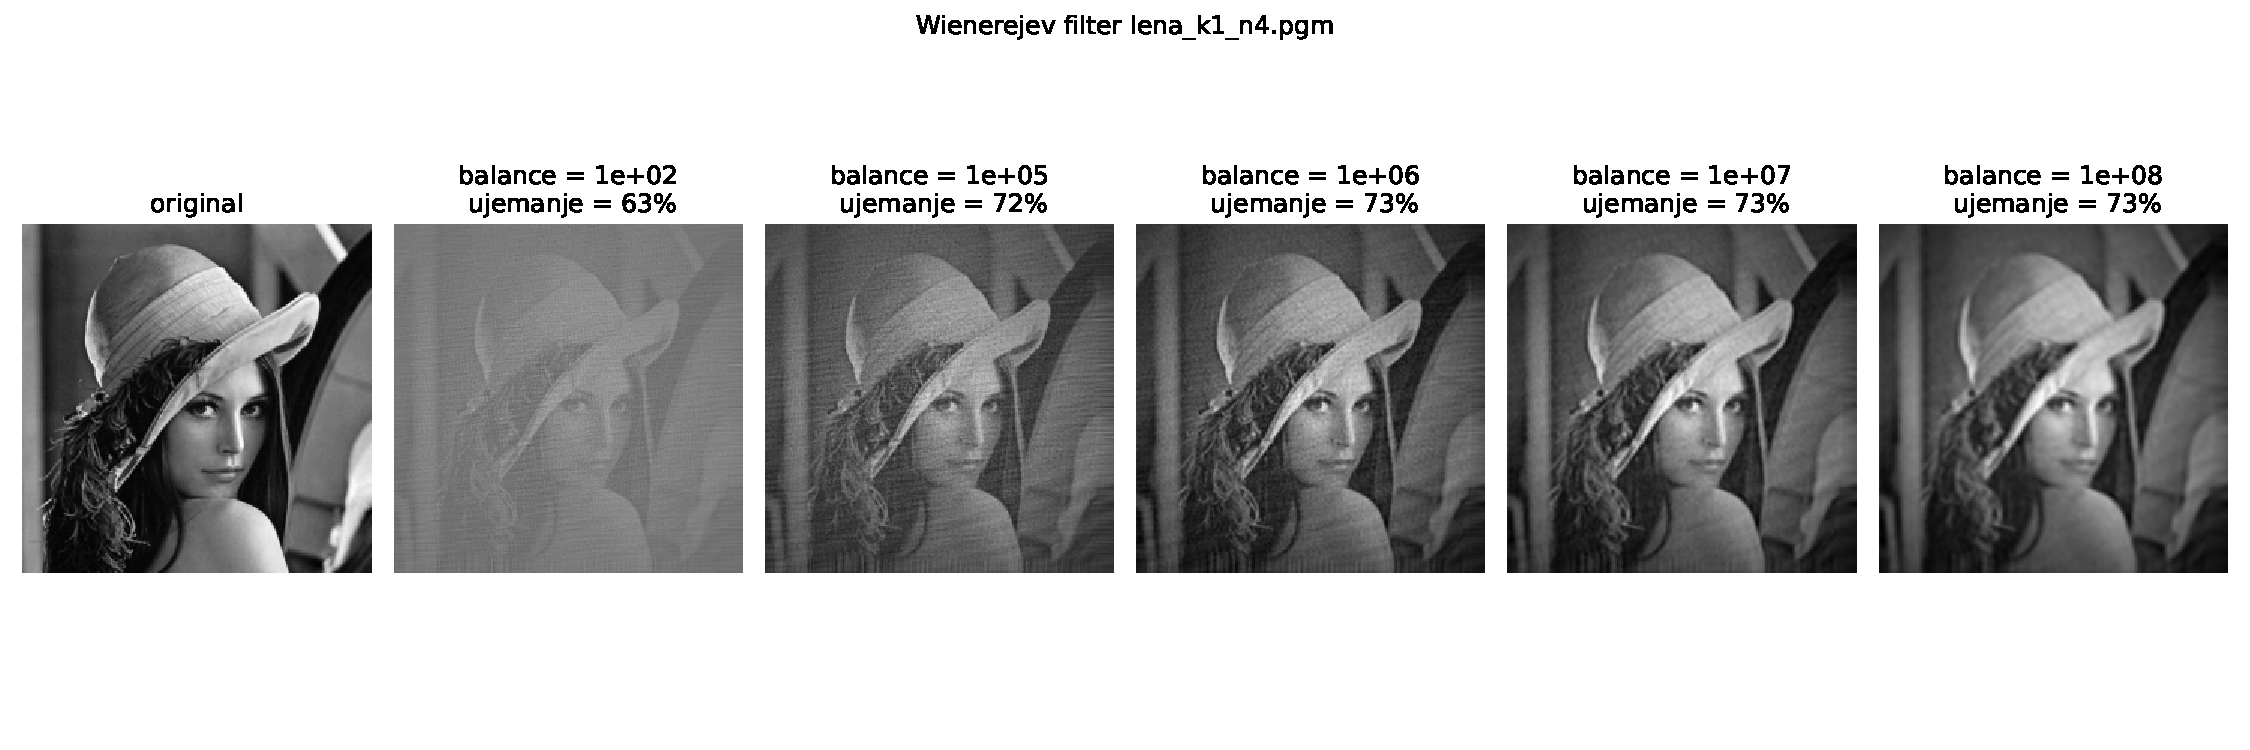
\includegraphics[width=\textwidth]{10.nal_slike/10.3/wiener_kernel1.pdf}
    \caption{Dekonvolucija zašumnljene slike \texttt{lena\_k1\_n4.pgm} z različnim prametrom \textit{balance} v Wienerejevem filtru}
\end{figure}

\newpage
Na tem mestu sem ugotovil, kako lahko umerim filter za kar najboljši rezultat, kar je predstavljeno v spodnji preglednici. Kot sem omenil že poprej, jedro 2 v splošnem rabi malenkost večji parameter, zanimivo je pri jedru 3, vendar je rezultat lep in boljši od konkurenčnih metod (Richardson-Lucy in unsupervised\_Wiener iz knjižnice \allowbreak \texttt{skimage.restoration}). Slednji iterativno in stohastično oceni parametre dekonvolucije, vendar je v splošnem slabši (in počasnejši) in Wienerja, če poznamo oceno šuma zanj. Tako dekonvoluirane slike v končni verziji so prikazane v prilogi.

\begin{table}[ht]
    \centering
    \begin{tabular}{c|c|c|c|c}
    kernel\textbackslash{}šum(RMS) & 0   & 4   & 8   & 16  \\
    \hline
    1                               & $10^6$ & $10^6$ & $10^7$ & $10^7$ \\
    \hline
    2                               & $10^6$ & $10^7$ & $10^8$ & $10^8$ \\
    \hline
    3                               & $10^0$ & $10^6$ & $10^6$ & $10^6$
    \end{tabular}
    \caption{Vrednosti parametra \textit{balance} za kar najboljšo filtracijo}
    \label{tab:balance}
\end{table}

Periodično motnjo sem napadel s taistimi metodami kot Gaussovski šum, vendar Wiener ni več tako uspešen, saj se periodične motnje pojavljajo tudi na dekonvoluirani sliki le še bolj izrazite. Presenečen pa sem, da se algoritem LR odziva enako kot na slike brez periodične motnje. Tudi ujemanja so podobna onim brez periodične motnje, čeprav manjša od Wienerjevih, vendar je slika vizualno lepša. Zanimivo, da je tudi izračun napake pri jedru 1 in algoritmu LR v tem primeru pravilno izračunan, takisto tudi v prilogi. Napake v kodi, ki bi bila kriva za anomalije na slikah \ref{fig:napaka} in \ref{fig:vse_brez_sum} nisem našel!

\begin{figure}[ht]
    \centering
    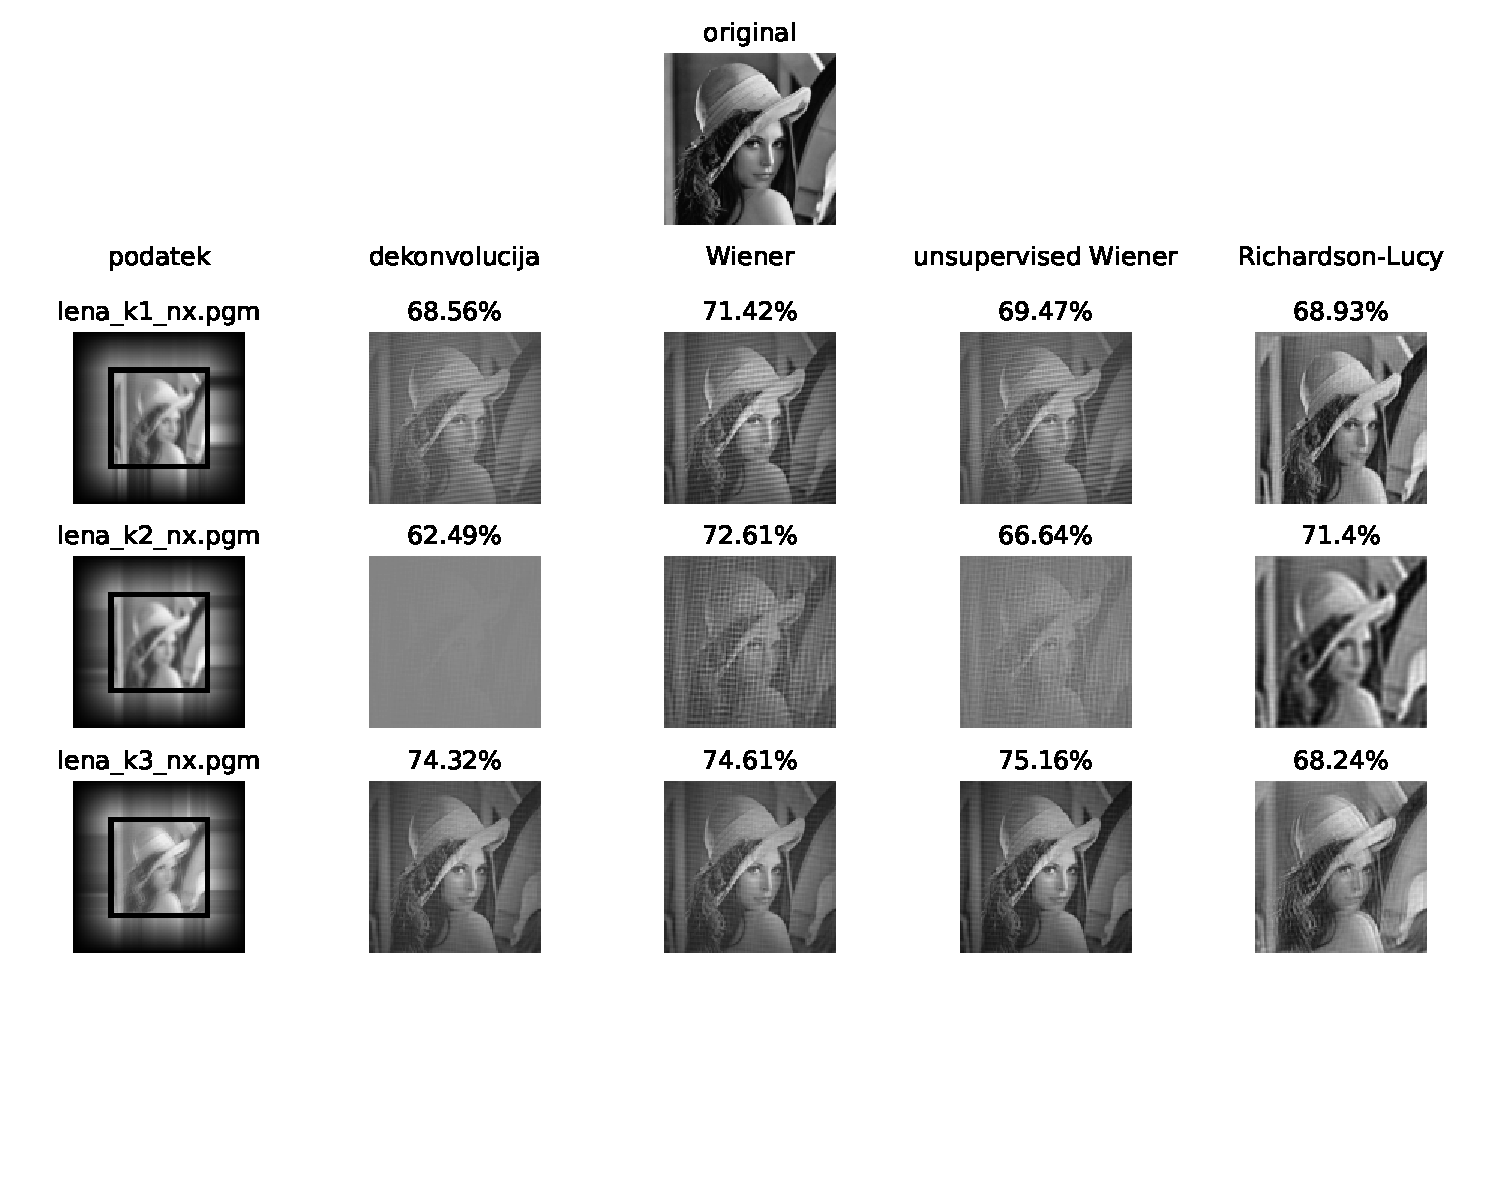
\includegraphics[width=\textwidth]{10.nal_slike/10.3/kernel_nx_vse.pdf}
    \caption{Poskus dekonvolucije slik s periodično motnjo}
\end{figure}

\newpage
\section{Priloga: končni rezultati dekonvolucije Lene}

\noindent
V vseh primerih je uporabljenih 200 px razširitve z linear\_ramp in okenska funkcija triang. Število iteracij algoritma Richardson-Lucy je 50, razen za jedro 3, kjer jih je 10. Parameter balance je tak, kot je ugotovljeno v tabeli \ref{tab:balance}.
\\
Pomembna opomba: Izračunane parametre ujemanja je potrebno jemati z rezervo, še vedno priporočam vizualno primerjavo!

\begin{figure}[ht]
    \centering
    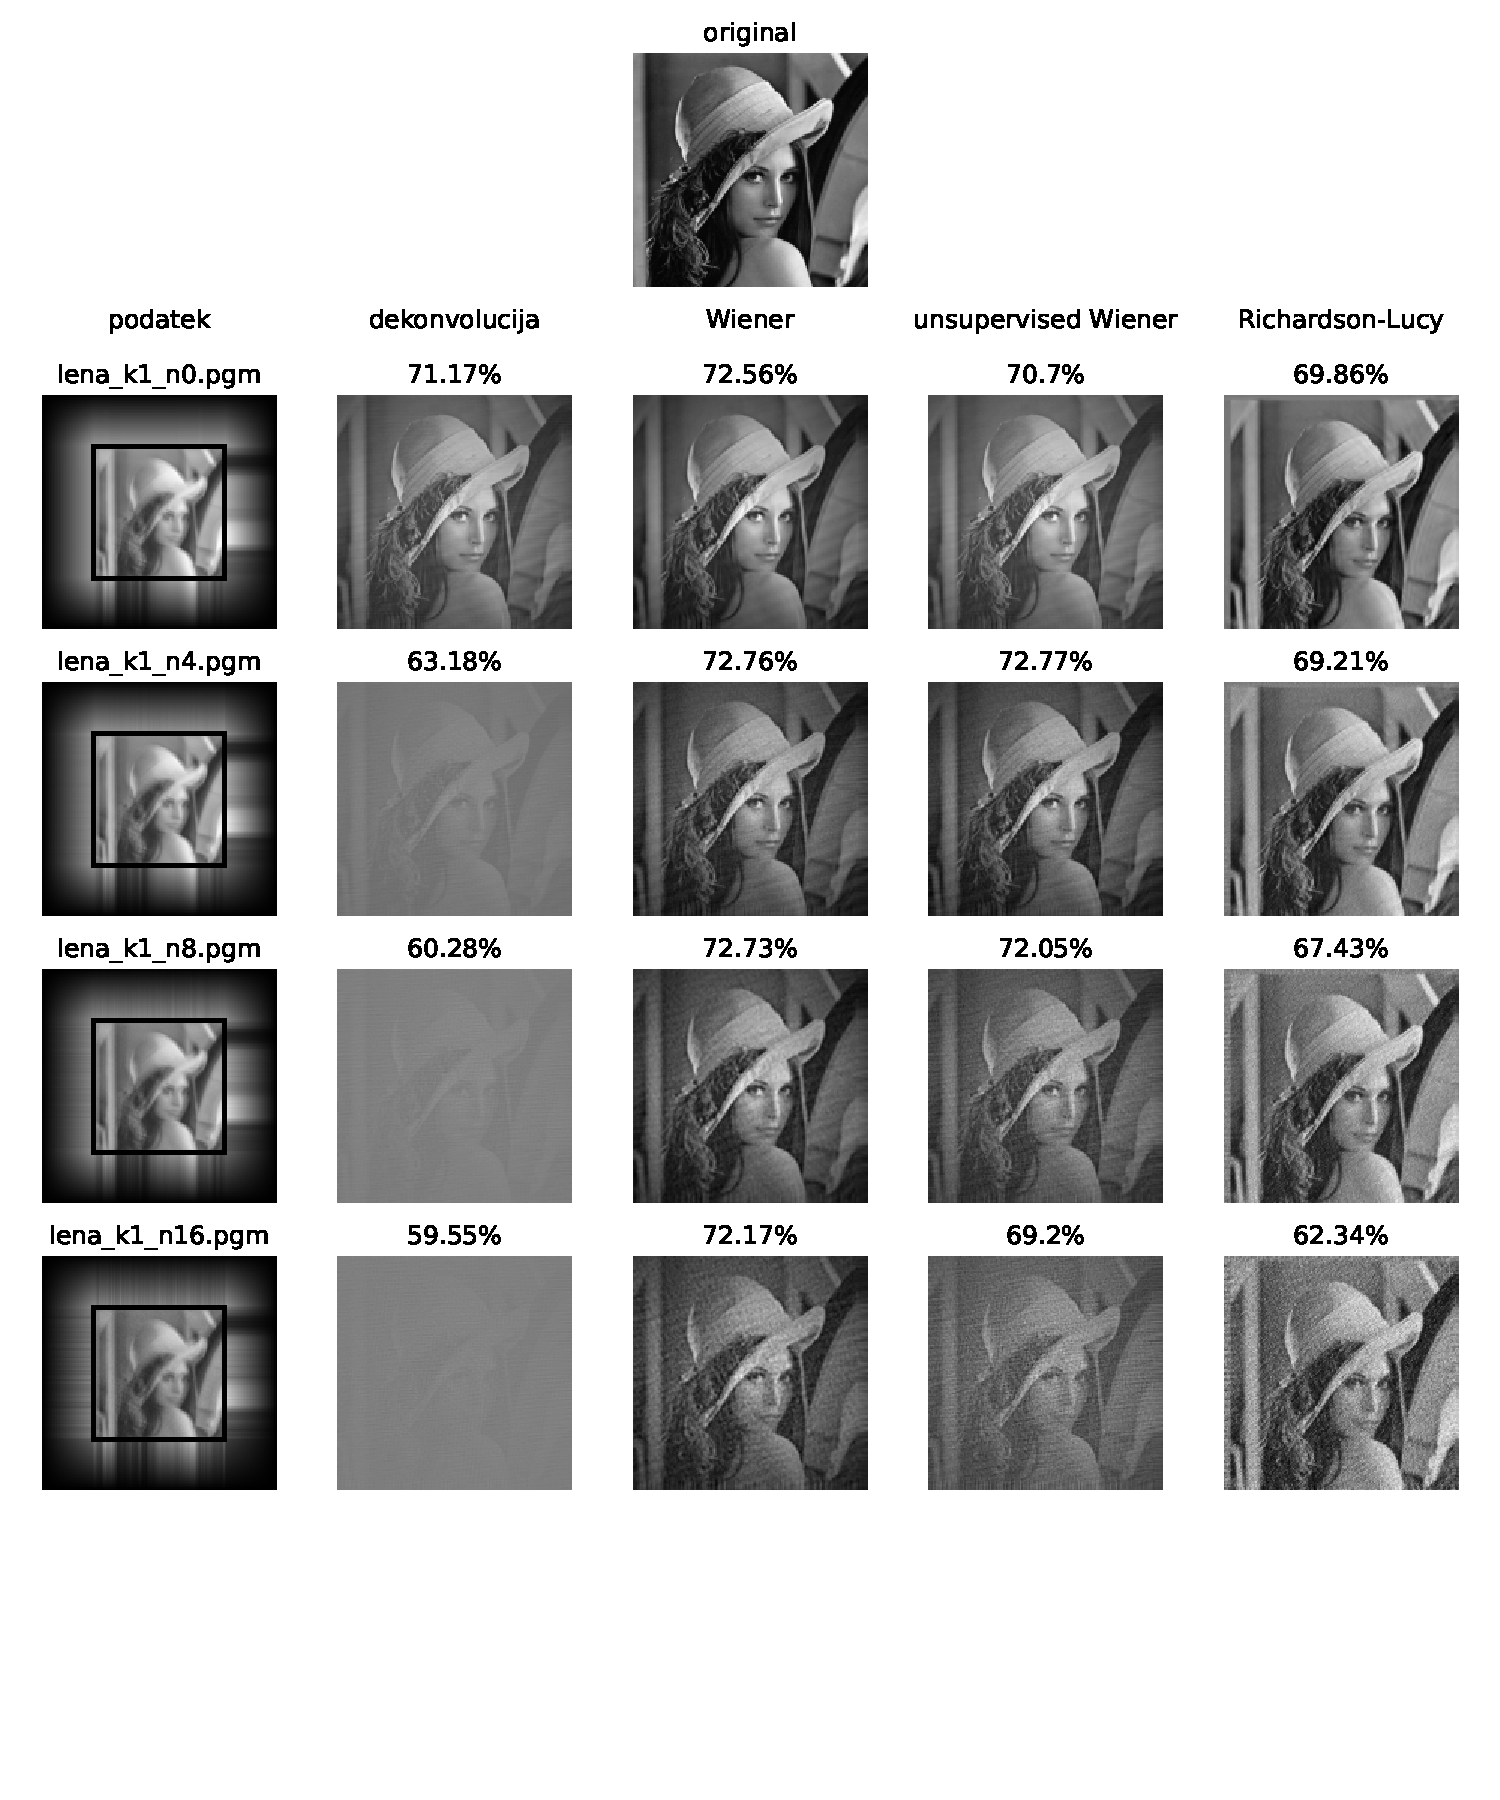
\includegraphics[width=\linewidth]{10.nal_slike/10.3/kernel1_wiener_vse.pdf}
    \caption{Kernel1}
\end{figure}
\begin{figure}[ht]
    \centering
    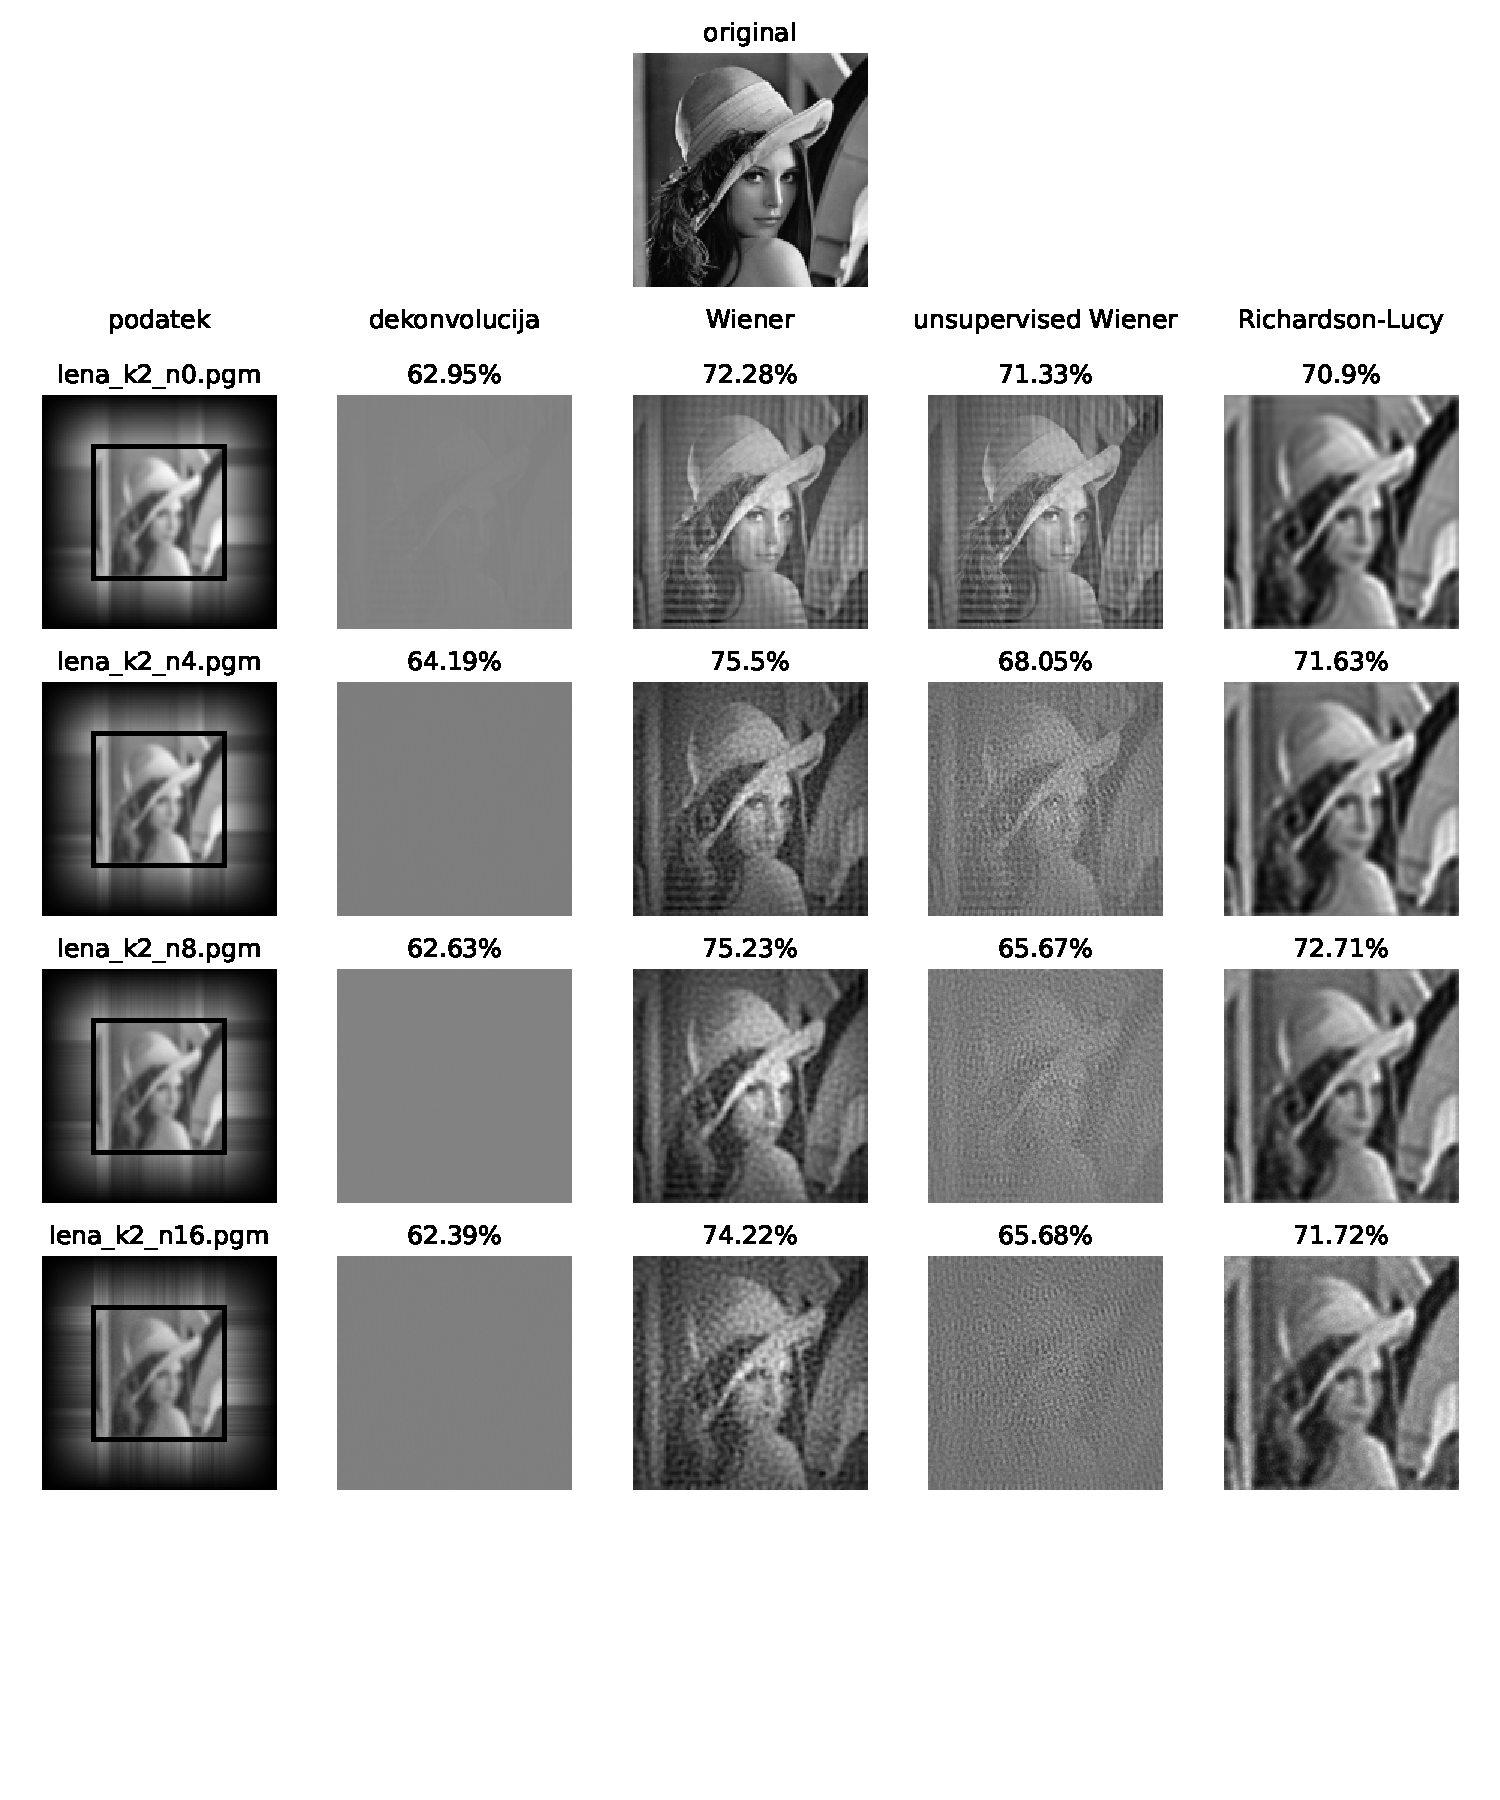
\includegraphics[width=\linewidth]{10.nal_slike/10.3/kernel2_wiener_vse.pdf}
    \caption{Kernel2}
\end{figure}
\begin{figure}[ht]
    \centering
    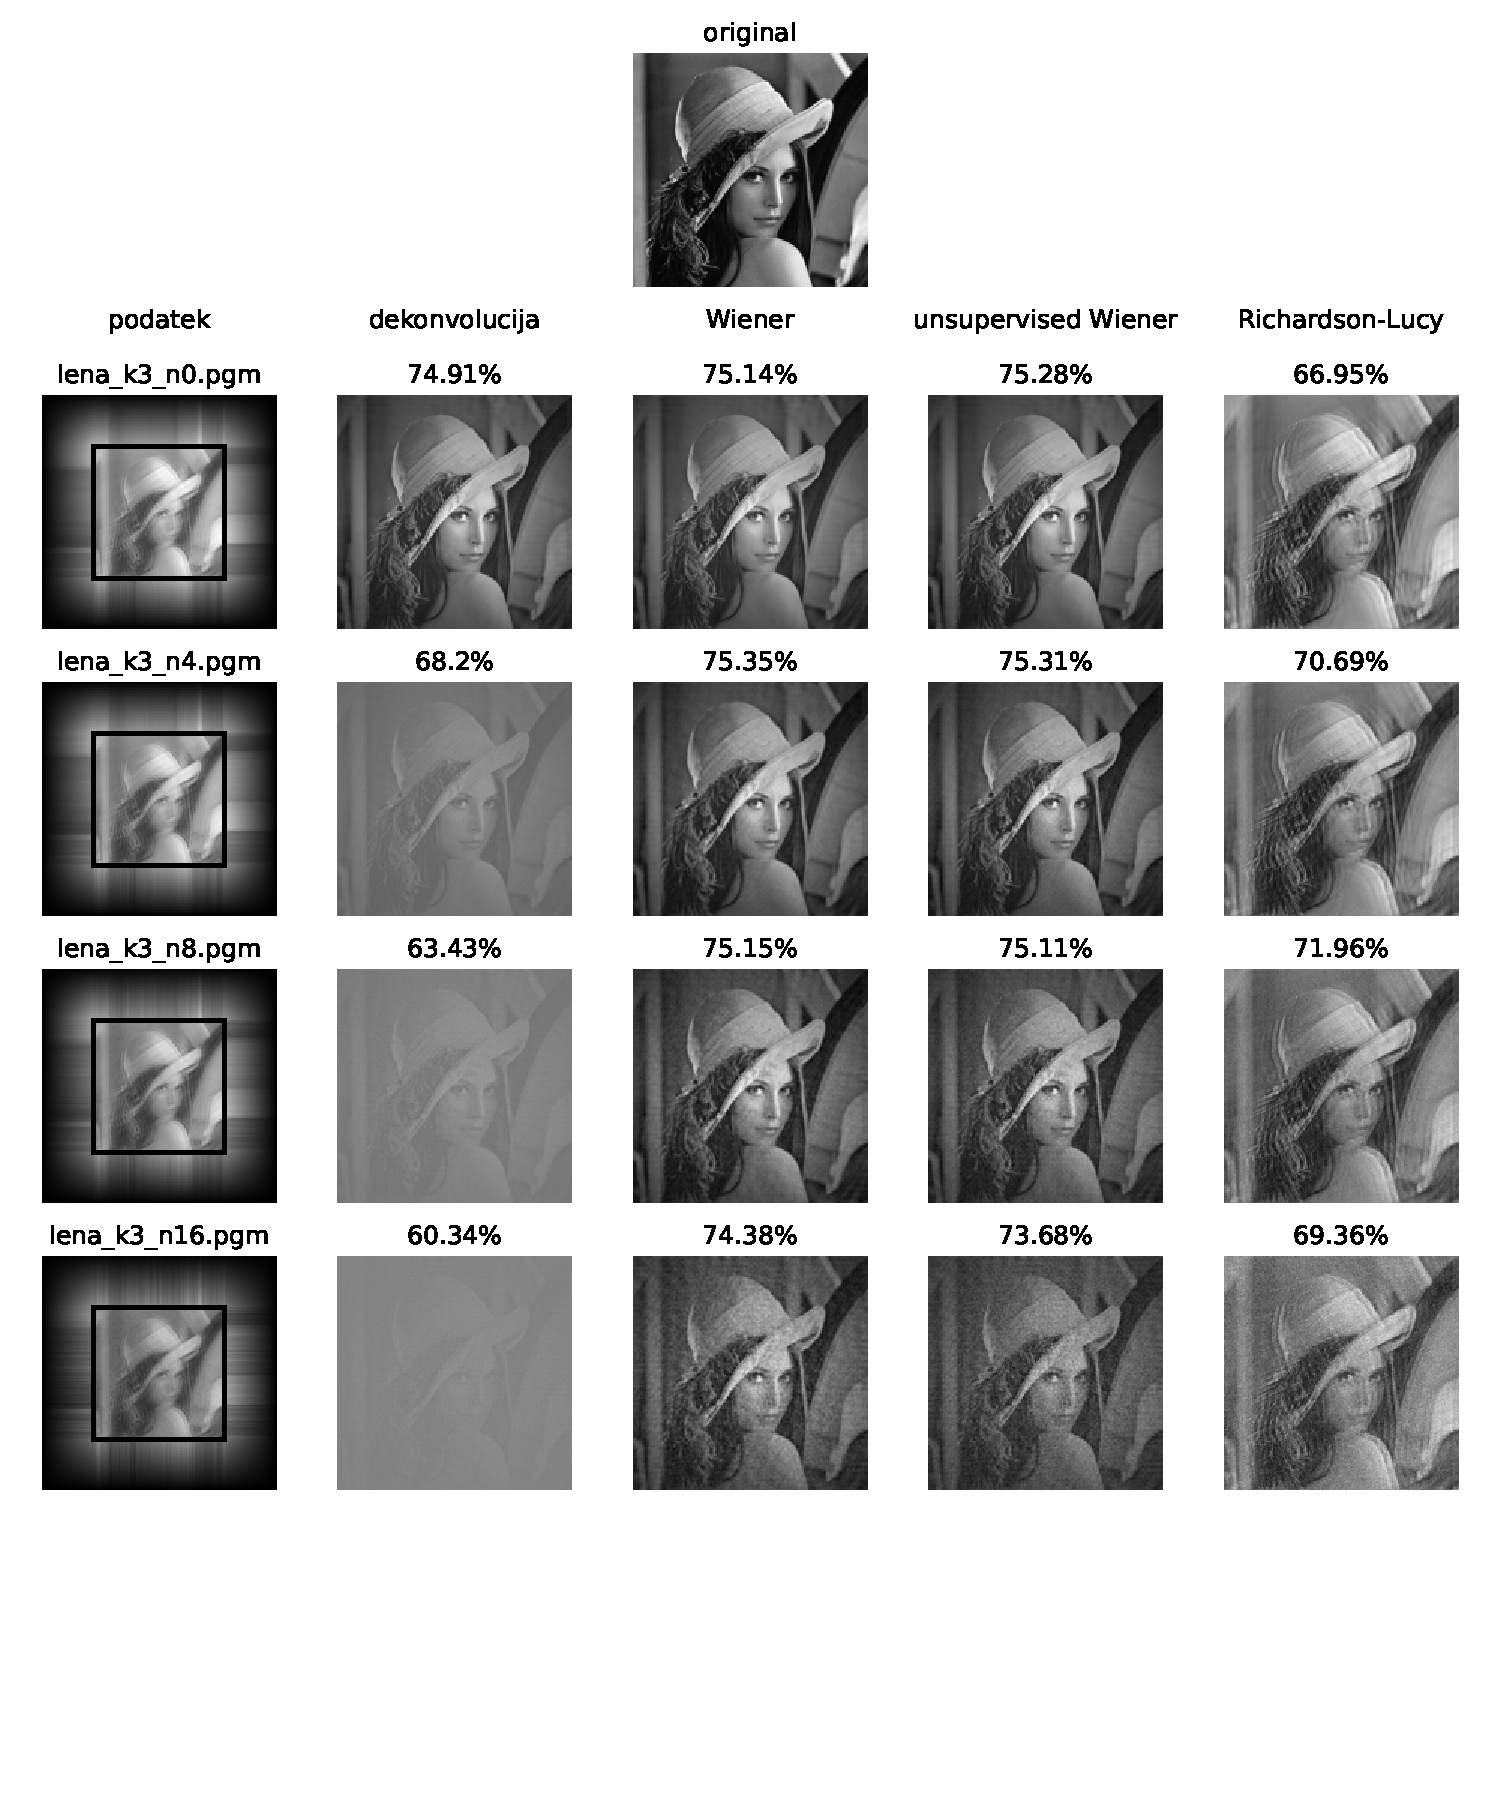
\includegraphics[width=\linewidth]{10.nal_slike/10.3/kernel3_wiener_vse.pdf}
    \caption{Kernel3}
\end{figure}
